\documentclass[7pt,landscape, margin = 0.1mm]{article}
\usepackage{amssymb,amsmath,amsthm,amsfonts}
\usepackage{bm}
\usepackage{multicol,multirow}
\usepackage{mathrsfs}
\usepackage{graphicx}
\usepackage{float}
\usepackage{calc}
\usepackage[dvipsnames]{xcolor}
\usepackage{ifthen}
\usepackage{titlesec}
\usepackage[landscape]{geometry}
\usepackage{enumitem}
\usepackage{syntonly}
\setitemize{noitemsep,topsep=0pt,parsep=0pt,partopsep=0pt}
\usepackage[colorlinks=true,citecolor=blue,linkcolor=blue]{hyperref}
\usepackage{tikz}
\def\cm{\tikz\fill[scale=0.4](0,.35) -- (.25,0) -- (1,.7) -- (.25,.15) -- cycle;} 
\ifthenelse{\lengthtest { \paperwidth = 11in}}
    { \geometry{top=.1in,left=.1in,right=.1in,bottom=.1in} }
	{\ifthenelse{ \lengthtest{ \paperwidth = 297mm}}
		{\geometry{top=1mm,left=1mm,right=1mm,bottom=1mm} }
		{\geometry{top=1mm,left=1mm,right=1mm,bottom=1mm} }
	}

\pagestyle{empty}

\makeatletter

 

\newcommand{\nextcol}{\vfill\null\columnbreak}

\newcommand{\titellinie}{\rule{1.\linewidth}{0.75pt}}

\titleformat{\subsection}
  {\normalfont\fontsize{10}{10}\bfseries}{\thesection}{1em}{}

\newcommand*{\mysection}[2][black]{\vskip 0pt \titellinie\vspace{-20pt}\section{#2}\vspace{-14pt}\titellinie \colorlet{chaptercolor}{#1}}

\newcommand*{\mysubsection}[1]{\vspace{-2mm}\color{chaptercolor}\subsection{ #1 }
\vspace{-1mm}\hrule\vspace{1.5mm}\color{black}
\vspace{2mm}}

\newcommand{\COL}[1]{ \color{chaptercolor} \bf{#1}\color{black}     \\}


\newcommand{\KRZ}[2]{\vspace{1mm} \hline \vspace{1mm} \color{chaptercolor}{RC #1}:\color{black} \   \hspace{0.2cm}\vspace{1mm}   {\begin{minipage}{20em}
#2 \end{minipage}} \vspace{1mm}  \hline \vspace{1mm}  \\}

\newcommand{\RC}[2]{\color{chaptercolor}\bf{RC #1}:\color{black}    \hspace{0.2cm} #2}

\newcommand{\DEF}[2]{\color{chaptercolor}\bf{Def #1}:\color{black}    \hspace{0.2cm} #2}

\newcommand{\NOTE}[2]{\color{chaptercolor}\bf{Note #1}:\color{black}    \hspace{0.2cm} #2 \\}

\newcommand{\COR}[2]{\color{chaptercolor}\bf{Cor #1}:\color{black}    \hspace{0.2cm} #2}

\newcommand{\LEM}[2]{\color{chaptercolor}\bf{Lem #1}:\color{black}    \hspace{0.2cm} #2 \\}

\newcommand{\THE}[2]{\color{chaptercolor}\bf{Trm #1}:\color{black}    \hspace{0.2cm} #2 \\}

\newcommand{\SA}[2]{\color{chaptercolor}\bf{S #1}:\color{black}    \hspace{0.2cm} #2}

\makeatother
\setcounter{secnumdepth}{0}
\setlength{\parindent}{0pt}
\setlength{\parskip}{0pt plus 0.5ex}
\setlength{\marginparwidth}{0pt}
\setlength{\marginparsep}{0pt}
% -----------------------------------------------------------------------
\begin{document}
%\syntaxonly
\centering

\scriptsize

\begin{center}
     \Large{\textbf{BSc. Computer Science - Linear Algebra - Boas Meier}}
\end{center}
\begin{multicols}{4}
\setlength{\premulticols}{0.5pt}
\setlength{\postmulticols}{0.5pt}
\setlength{\multicolsep}{0.5pt}
\setlength{\columnsep}{0.2pt}
\setlength{\columnseprule}{0.4pt}
\setlength{\intextsep}{0pt}

\begin{flushleft}


\mysection[BurntOrange]{\centering SLE}
\mysubsection{Gauss Algorithm}

\begin{figure}[H]
 \centering
 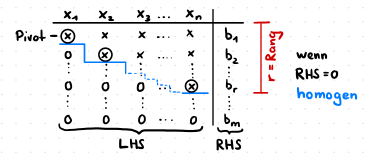
\includegraphics[scale=1]{pictures/Gauss.png} 
\end{figure}

\color{chaptercolor} Compability Conditions: \color{black} $b_{r+1}=...=bm=0$

\SA{1.1}{$Ax = b $ hat min eine Lösung $\Leftrightarrow r = m $ oder $ r<m + \color{chaptercolor} VB \color{black}$ dann:  $ r=n \Leftrightarrow  1 $ Lösung , $ r<n \Leftrightarrow \infty $ Lösungen}

\SA{}{Row-operations preserve (in)dependence of columns. Proof: columns of $A$ are dependent $\Leftrightarrow \exists x \not = \bm{0}$ s.t. $Ax=\bm{0} \Leftrightarrow \exists x\not =\bm{0}$ s.t. $A' x=\bm{0} \Leftrightarrow$ columns of $A'$ are dependent.}

\SA{}{Gauss elimination succeeds $\Leftrightarrow$ the columns of $A$ are independent $\Leftrightarrow$ A has full rank.}

\COR{}{For a quadratic SLE $Ax=b$ ($A$ is $n \times n$ $\Rightarrow n$ equations and $n$ variables) we have the following set of equivalence, of which ONLY one of them can be true; So, EITHER
\begin{itemize}
 \item[i] $rank(A) = n \Leftrightarrow A$ is regular
 \item[ii] for every $b \in \mathbb{R}^n$, $Ax=b$ has a unique solution $x=A^{-1}b$
 \item[iii] the corresponding homogeneous system has only the trivial solution 
 \end{itemize}
 OR the following equivalences hold
\begin{itemize}
 \item[v] $rank(A) < n \Leftrightarrow A$ is singular
 \item[vi] for some $b$ there exists no solution
 \item[vii] for no $b$ a unique solution exists
 \item[viii] for some $b$ infinity many solution exists
 \item[ix] the corresponding homogeneous system has non-trivial solutions
\end{itemize}}

\mysubsection{Gauss-Jordan Algorithm}

\mysection[Dandelion]{\centering Matrices and Vectors}
\mysubsection{Definitions}
A $m \times n  $ matrix has m \COL{row (Zeilen)$\downarrow$}  and n \COL{columns (Spalten)$\to$}, in which the i,j element gets noted by $a_{i,j}$ or $(A)_{i,j}$

\DEF{nullmatrix}{$a_{i,j}=0\ \forall\ i,j$}

\DEF{diagonalmatrix}{Has in every entry $0$ except for the diagonal: $(A)_{ij} = 0$ for $i \neq j $ one can write $diag(d_{11}, \cdots , d_{nn})$. It holds that
\begin{enumerate}[nolistsep]
    \item is symmetric
    \item $det(A)=\prod_{i=1}^n A_{ii}$
    \item $A^{-1}=diag(\frac{1}{A_{11}}, \cdots, \frac{1}{A_{nn}})$
    \item $A^m=diag(A_{11}^m, \cdots, A_{nn}^m)$
    \item values in the diagonal are the eigenvalues and the canonical basis is a set of eigenvectors.
\end{enumerate}

\DEF{identity}{The identity is written as $I_n = diag(1 , \cdots , 1)$. It holds that $AI = IA = A$ and $I^{-1}=I$.}

\DEF{upper triangular matrix}{We have $(R)_{ij} = 0$ for $i > j $ (Rechtsdreiecksmatrix).}

\DEF{lower triangular matrix}{We have $(R)_{ij} = 0$ for $i < j $ (Linksdreiecksmatrix).}

\SA{Facts about triangular matrices}{\begin{enumerate}[nolistsep]
    \item are nilpotent
    \item the product of two upper(lower)-triangular matrices is as well upper(lower)-triangular.
    \item the inverse of a upper(lower)-triangular matrix is as well upper(lower)-triangular.
    \item values in the diagonal are the eigenvalues.
\end{enumerate}}

\DEF{Matrix-set}{The set of $ m \times n $-matrices is written as: $\mathbb{E}^{m \times n } $ For vectors we have: $ \mathbb{E}^{n}$, where $ \mathbb{E}$ is $ \mathbb{R}$ or $ \mathbb{C}$}

\DEF{matrix multiplication}{If $C =AB $ then one can write $C_{ij} = (AB)_{ij} = \sum_{k=1}^{n} (A)_{ik}(B)_{kj} = \sum_{k=1}^{n} a_{ik}b_{kj}$}

\SA{Calculation Rules for Vectors}{
Let $v,w,u \in \mathbb{E}^n$ with $\mathbb{E}$ being an arbitrary vector space and $n \in \mathbb{N}$. Let $\lambda,\mu \in \mathbb{R}$. Let $\bm{0}$ be the nullvector. Axioms of vector spaces:
\begin{enumerate}[nolistsep]
 \item $v+w=w+v$
 \item $(v+w)+u= v+(w+u)$
 \item $v+\bm{0}=v$
 \item $v+(-v)=\bm{0}$
 \item $\lambda (v+w)= \lambda v + \lambda w$
 \item $(\lambda + \mu)v= \lambda v + \mu v $
 \item $(\lambda \mu)v= \lambda (\mu v) = \mu (\lambda v)$
 \item $1v=v$
\end{enumerate}}

\SA{Linear Combination}{Let $v_i \in \mathbb{R}^m$ with $m \in \mathbb{N}$ for $i \in \{1, ..., n\}$. Then
$c_1v_1 + c_2v_2 + ... + c_n v_n = b \iff \stackrel{(m \times n)}{\begin{bmatrix}
| &  & |\\
v_1 & ... & v_n\\
| &  & |
\end{bmatrix}} \stackrel{(n \times 1)}{\begin{bmatrix}
c_1\\ \vdots\\ c_n
\end{bmatrix}} = \stackrel{(m \times 1)}{\begin{bmatrix}
|\\ b\\ |
\end{bmatrix}
}$}

\DEF{Zerodiviser}{If $AB=0 \iff $ A,B Zerodiviser, Nullteiler}

\DEF{transposes}{ $ (A^T)_{ij}=A_{ji} $}

\DEF{conjugate transposed}{$ A^H = (\overline{A})^T=\overline{A^{T}}$}

\DEF{symmetric}{$A^T = A \Leftrightarrow $A symmetric $\Leftrightarrow A$ is square.
\begin{enumerate}[nolistsep]
    \item for every matrix $A$, both $A^TA$ and $AA^T$ are symmetric, PSD, and have the same non-zero eigenvalues.
    \item Let $AB$ be symmetric. Then $AB=BA$.
    \item if positive definite $\Rightarrow$ regular (check)
\end{enumerate}

\DEF{skew-symmetric}{$A^T = -A  \iff $A skew-symmetric}

\DEF{hermitian}{$A^H = A  \iff $A hermitian}

\DEF{invertible}{$A$ is invertible $\Leftrightarrow A$ is regular $\Leftrightarrow \exists A^{-1} \Leftrightarrow A^{-1}A=AA^{-1}=I \Leftrightarrow A^{-1}$ is unique}

\SA{}{If $A, B$ are regular: \begin{enumerate}[nolistsep]
  \item $A^{-1}$ is regular
  \item $AB$ and $BA$ are regular
  \item $A^T$ is regular
  \item $A^TA$ is regular
  \item $A^k$ is regular and $(A^k)^{-1}=(A^{-1})^k$.
\end{enumerate}}

\DEF{nilpotent}{A matrix $A$ is said to be nilpotent if $A^k = 0$ with $k \in \mathbb{N}$. Always $A^0=I$.}

\SA{Calculation Rules for Matrices}{
\begin{enumerate}[nolistsep]
 \item $A+B=B+A$\\ $AB \neq BA$
 \item $(A+B)+C= A+(B+C)$\\ $(AB)C=A(BC)$
 \item $A+\bm{0}=A$\\ $AI=IA=A \iff$ A is square
 \item $AB=\bm{0} \not\Rightarrow A=\bm{0} \lor B=\bm{0}$
 \item $AB=AC \not\Rightarrow B=C$
 \item $\lambda (A+B)= \lambda A + \lambda B$ with $\lambda \in \mathbb{R}$
 \item $A(B+C)=AB+AC$
 \item $(A+B)C=AC+BC$
 \item $(A^{-1})^{-1}=A$
 \item $(AB)^{-1}=B^{-1}A^{-1}$\\$(ABC)^{-1}=C^{-1}B^{-1}A^{-1}$
 \item $(A^T)^T=A$
 \item $(A+B)^T=A^T+B^T$
 \item $(AB)^T=B^TA^T$
 \item $(A^{-1})^T=(A^T)^{-1}$
\end{enumerate}

\SA{Finding an inverse}{
\begin{enumerate}[nolistsep]
 \item[15a.] $M=\begin{bmatrix}
     x
 \end{bmatrix}, M^{-1}=\begin{bmatrix}
     \frac{1}{x}
 \end{bmatrix}$ (if $x \not = 0$)
 \item[15b.] $M=\begin{bmatrix}
     a & b\\
     c & d
 \end{bmatrix}, M^{-1}=\frac{1}{ad-bc}\begin{bmatrix}
     d & -b\\
     -c & a
 \end{bmatrix}$ (if $ad-bc \not = 0$)
 \item[15c.] $[M|I] \xrightarrow[op]{row}[I|M^{-1}]$
 \item[15d.] $ A =  \left[ 
 \begin{array}{c|c} 
  a_{11} & a_{12} \\ 
  \hline 
  a_{21} & a_{22} 
 \end{array} 
 \right] \Leftrightarrow A^{-1} = \left[ 
 \begin{array}{c|c} 
  a_{11}^{-1}  & a_{12}^{-1}  \\ 
  \hline 
  a_{21}^{-1}  & a_{22} ^{-1} 
 \end{array} 
 \right] $
 \end{enumerate}
}}


\mysubsection{Scalar Product and Norm}
\DEF{Outer Product}{m-vector $x$ and n-vector $y$: $xy^T$}

\SA{}{A $m \times n $-matrix has rank 1 if it is the outer product of an m-vector $\neq 0 $ and n-vector $\neq 0 $}

\DEF{Scalar Product (Dot Product, Inner Product)}{ $\left<v,w\right> = v^Tw = \sum_{i=1}^{n} \overline{v_i} w_i \xrightarrow[ \mathbb{R}]{in}\sum_{i=1}^{n} v_i w_i$}

\SA{Calculation Rules for Scalar Product}{\begin{enumerate}[nolistsep]
  \item $v^T(w+u)=v^Tw+v^Tu$ (linear in 2nd factor)
  \item $v^T(\lambda w) = \lambda v^Tw$ (linear in 2nd factor)
  \item $(v+w)^Tu=v^Tu+w^Tu$ 
  \item for $ \mathbb{E} = \mathbb{R}$: $ (\lambda v)^Tw= \lambda (v^Tw)$ (linear in 1st factor)\\ for $ \mathbb{E} = \mathbb{C}$: $(\lambda v)^Tw = \overline{\lambda}\ (v^Tw)$ (conjugate-linear in 1st factor)
  \item for $ \mathbb{E} = \mathbb{R}$: $v^Tw=w^Tv$ (symmetric)\\ for $ \mathbb{E} = \mathbb{C}$: $v^Tw=\overline{w^Tv}$ (hermitian)
  \item $v^Tv > 0, v^Tv=0 \iff v=\bm{0}$ (positive definite)
\end{enumerate}
}

\DEF{norm}{$ \|v\| = \sqrt{v^Tv} = \sqrt{\sum_{i=1}^{n} (|v_i|)^2} \xrightarrow[\mathbb{R}]{in} \sqrt{\sum_{i=1}^{n} v_i^2}$}

\DEF{}{$\cos(\alpha)$ between $v,w$: $ \cos(\alpha) = \frac{Re (v^Tw)}{\|v\| \cdot \|w\|}\xrightarrow[\mathbb{R}]{in} \frac{v^Tw}{\|v\| \cdot \|w\|}$}

\SA{Cauchy-Schwarz inequality (because $cos(\alpha)\leq 1$)}{$|v^Tw| \leq \|v\| \cdot \|w\|$("=" holds when $w$ is a multiple of $v$ or vice versa)}\\

\DEF{Cauchy-Bunyakovsky-Schwarz}{Cauchy-Schwarz inequality squared yields: $|v^Tw|^2 \leq \|v\|^2 \cdot \|w\|^2 = (v^Tv) \cdot (w^Tw)$}

\SA{Properties of the Norm}{
\begin{enumerate}[nolistsep]
  \item $\|v\| > 0, \|v\| = 0 \iff v=0$ (positive definite)
  \item $\|\lambda v\| = \lambda \|v\| $ (homogeneous)
  \item $\|v + w\| \leq \|v\| + \|w\|$ (Triangle-inequality)
\end{enumerate}} 

\DEF{orthogonal}{$v,w$ are orthogonal $\Leftrightarrow v^Tw=0 \Leftrightarrow v \perp  w \Leftrightarrow \|v + w\|^2 =\|v\|^2 + \|w\|^2$ (Pythagoras)}

\DEF{orthonormal}{The vectors $q_1,...,q_n\in\mathbb{R}^m$ are orthonormal if they are orthogonal and have norm 1. Let $\delta_{ij}=$
\begin{cases}
    0 & \text{if $i\not=j$}\\
    1 & \text{if $i=j$}
\end{cases} be the Kronecker delta. Then $q_i^Tq_j=\delta_{ij}$ $\forall i,j=1,...,n \Leftrightarrow Q^TQ=I$.}

\DEF{Hyperplane}{If $d \in \mathbb{R}^n, d \not= 0$, then $\{v\in \mathbb{R}^n | v^Td=0\}$ (all vectors perpendicular to $d$) is a hyperplane.

\DEF{Manhattan Distance (p-norm)}{$\left\|x\right\|_p = (\sum_{i=1}^n|x_i|^p)^{\frac{1}{p}}=\left ( \left| x_1 \right|^p \cdots \left| x_n \right|^p \right )^{\frac{1}{p}}$ for $1\leq p < \infty$, and $||x||_\infty=max_i|x_i|$.}

\DEF{Frobenius Norm}{Let $A\in\mathbb{R}^{m\times n}$. Then $||A||_F=\sqrt{\sum_{i=1}^m\sum_{j=1}^nA_{ij}^2}$.}

\DEF{Operator (or spectral) Norm}{Let $A\in\mathbb{R}^{m\times n}$. Then $||A||_{op}=\underset{\underset{s.t.||x||=1}{x\in\mathbb{R}^n}}{max}||Ax||$.}

\SA{}{Let $\sigma_1\leq...\leq\sigma_{min(n,m)}$ be $A$'s singular values. Then
\begin{enumerate}[nolistsep]
    \item $||A||_F^2=Tr(A^TA)=\sum_{i=1}^n\sigma_i^2$
    \item $||A||_{op}=\sigma_1$
    \item $||A||_{op}\leq||A||_F\leq\sqrt{min\{m,n\}}||A||_{op}$
\end{enumerate}}

\mysubsection{Linear Dependency and Rank}
\DEF{Linear Dependency}{Vectors $w_1, w_2, ..., w_k$ are linearly independent $\Leftrightarrow$ no vector is a combination of the other ones $\Leftrightarrow$ there are no $c_1, c_2, ...,c_k$ besides $0, 0, ..., 0$ s.t. $c_1w_1 + c_2w_2 + ... + c_kw_k = \bm{0}$.}

\DEF{Rank}{Let $A\in\mathbb{R}^{m\times n}$. $rank(A) =$ \# of independent columns of $A =$ \# of independent rows of $A$. \begin{enumerate}[nolistsep]
    \item if full rank\: $r=min(m,n)$ else $r \leq min(m,n)$.
    \item $rank(A)=rank(A^T)=rank(A^TA)=rank(AA^T)$.
\end{enumerate}}}

\mysubsection{A = CR}
Let $r=rank(A)$.
$A=\stackrel{(m \times n)}{\begin{bmatrix}
1 & 2 & 0 & 3\\
2 & 4 & 1 & 4\\
3 & 6 & 2 & 5
\end{bmatrix}}=\stackrel{(m \times r)}{\begin{bmatrix}
1 & 0\\
2 & 1\\
3 & 2
\end{bmatrix}}\stackrel{(r \times n)}{\begin{bmatrix}
1 & 2 & 0 & 3\\
0 & 0 & 1 & -2
\end{bmatrix}}=CR$
$C$: the independent columns of $A$ ($rank(C)=r$). If column $i$ of $R$ contains a unit vector, then column $i$ of $A$ is a column of $C$.\\
$R$: how to combine the independent columns to get all columns ($rank(R)=r$).


\mysubsection{\centering Orthogonal Matrices}
\DEF{orthogonal matrix}{A square matrix $Q\in\mathbb{R}^{n\times n}$ is an orthogonal matrix if $Q^TQ=I$. In this case, $QQ^T=I$, $Q^{-1}=Q^T$, and the columns of $Q$ form an orthonormal basis for $\mathbb{R}^n$.}

\SA{}{Images from orthonormal matrices are isometric and conformal (längen-winkeltreu). Hence norm and scalar product of vectors is preserved. In other words: $Q\in\mathbb{R}^{n\times n}$ is orthogonal $\Leftrightarrow ||Qx||=||x|| \land (Qx)^T(Qy)=x^Ty$ $\forall x,y\in\mathbb{R}^n$.}

\SA{}{Examples for orthogonal matrices are permutation and rotation matrices.}

\DEF{2d rotation}{\\
Counterclockwise: $R(\phi) = \begin{pmatrix}
cos \phi & -sin \phi \\
 sin \phi & cos \phi  \\
\end{pmatrix}$. 
Clockwise: $R(\phi) = \begin{pmatrix}
cos \phi & sin \phi \\
 -sin \phi & cos \phi  \\
\end{pmatrix}$}

\DEF{3d rotation}{$R_x(\phi) = \begin{pmatrix}
 1&0  &0  \\
 0& cos \phi  & -sin \phi  \\
 0& sin \phi  &  cos \phi \\
\end{pmatrix}\\
R_y(\phi) = \begin{pmatrix}
 cos \phi &0  &sin \phi  \\
 0&  1&0   \\
 -sin \phi& 0  &  cos \phi \\
\end{pmatrix}\\
R_z(\phi) = \begin{pmatrix}
  cos \phi& -sin \phi  &0  \\
 sin \phi& cos \phi  & 0  \\
 0& 0  &   1\\
\end{pmatrix} $}

\mysubsection{PA=LU Decomposition}
The LU-decomposition is useful when multiple SLE have the same A. Note that $EPA=U \Leftrightarrow PA=E^{-1}U \Leftrightarrow PA=LU \Leftrightarrow L=E^{-1} \implies PAx=LUx=Lc=Pb \Leftrightarrow Ux=c$.

\begin{itemize}
\item Find $L,U$ using row-operations on PA ($PA=E^{-1}U=LU$)
\item Solve $Lc=Pb$ for $c$ using back-substitution.
\item solve $Ux=c$ for $x$ using back-substitution.
\end{itemize}

\begin{figure}[H]
\centering
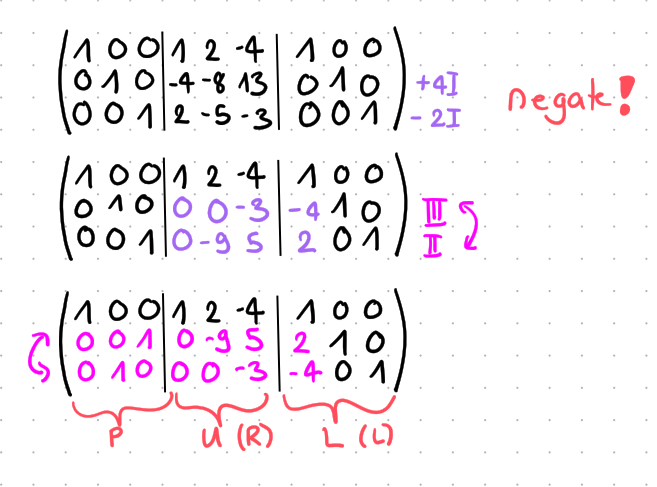
\includegraphics[scale=0.5]{pictures/LU-decomposition.png} 
\end{figure}

\COR{}{L is lower-triangular and U is upper-triangular.}

\mysubsection{$A=LDL^T$ (Symmetric LU)}
\DEF{}{$U=L^{-1}A \Leftrightarrow D=U(L^{-1})^T=U(L^T)^{-1}=L^{-1}A(L^T)^{-1}$ and $A=LU \Leftrightarrow A=LDL^T \Leftrightarrow U=DL^T$}

\SA{}{D is upper-triangular and symmetric $\Leftrightarrow$ D is diagonal}

a

\mysection[JungleGreen]{\centering Vectorspaces}
\DEF{}{A vectorspace $V$ over $\mathbb{K}$ is a non-empty set on which vector addition and scalar multiplication is defined. The operation of vector addition and scalar multiplication must satisfy the axioms of vector spaces.}

\SA{Properties of Vectorspaces}{In a vectorspace the following holds for a scalar $\alpha$ and vector $x \in V$: \begin{enumerate}[nolistsep]
 \item $0x = \bm{0}$
 \item $0\alpha = 0$
 \item $\alpha x = \bm{0} \Rightarrow \alpha = 0$ or $x = \bm{0}$
 \item $(-\alpha)x = \alpha(-x) = -(\alpha x)$
\end{enumerate}}

\DEF{polynomial space}{$\mathcal{P}_n$ is defined as all polynomials of degree $n$. Further: $ \mathcal{P} = \bigcup_{n=0}^{\infty} \mathcal{P}_n $}

\SA{}{$\{ b_1 , \cdots , b_n\} \subset V$ is a basis of V $\Leftrightarrow $ every vector $x \in V$ can be uniquely represented as: $x = \sum_{k=1}^{n}\xi_k b_k $}

\SA{}{$\forall x \in V, \forall y \in V \exists z \in V: x+z=y$ where $z$ is unique and $z = y + (-x) $}

\mysubsection{Subspace}
\DEF{}{A subspace (unterraum) $U$ is a non-empty subset of $V$ that is closed under vector addition and scalar multiplication and contains the $\bm{0}$ vector. Hence, let $v,w \in U$ and $c$ be scalar then $U \subseteq V \Leftrightarrow v+w \in U \land cv \in U \land cv+dw \in U \land \bm{0} \in U$.}

\SA{}{Every subspace is a vectorspace.}

\DEF{spanning set}{The vectors $v_1 , \cdots , v_n$ are a spanning set (erzeugendes System) of $V$, if $\forall w \in V \Leftrightarrow w \in span \{ v_1 , \cdots , v_n \}$.}

\COR{Examples of Subspaces of $V$}{\begin{enumerate}[nolistsep]
    \item $V=R^2$: Line through $\bm{0}$
    \item $V=R^3$: Plane through $\bm{0}$
    \item $V=R^(2 \times 2)$: all symmetric matrices, all diagonal matrices
\end{enumerate}}

\DEF{Column Space}{Let $A$ be $(m \times n)$. The column space (Spaltenraum) of $A$ is the subspace $C(A)=\{Ax|x\in \mathbb{R}^n\} = span(a_1, ..., a_n) = span(c_1, ..., c_r) \subseteq \mathbb{R}^m$ where $a_1, ..., a_n$ are the columns $A$ and $c_1, ..., c_r$ the $r$ independent columns of $A$. $dim(C(A))=rank(A)=r$}

\DEF{Row Space}{$R(A)=C(A^T)=C(A^TA)=R(R_0)=R(R)$ and $dim(R(A))=rank(A)=r$}

\DEF{Nullspace}{Let $A=CR$ be $(m\times n)$. The nullspace (Nullraum) of $A$ is the subspace $N(A)=\{x \in \mathbb{R}^n | Ax=\bm{0}\}=N(A^TA)=N(R)$. If all columns independent then $N(A)=\{\bm{0}\}$. $dim(N(A))=n-r$}

\DEF{Left Nullspace}{$N(A^T)=\{y \in \mathbb{R}^m | A^Ty=\bm{0}\}=\{y \in \mathbb{R}^m | y^TA=\bm{0}^T\}$ and $dim(N(A^T))=m-r$}

\COL{Computing the Nullspace by Elimination}
\begin{enumerate}[nolistsep]
    \item Find $A=CR$ using Gauss-Jordan.
    \item Read a basis of $N(R)$ off $R$. Basis consists of $n-r$ vectors.
\end{enumerate}
Let $R$ be $(r \times n)$. Let $X_I =$ the $r$ variables for $e_1, ..., e_r$ and $X_F =$ the $n-r$ others (free variables). Then $Rx=I_rX_I+FX_F=\bm{0} \Leftrightarrow X_I = -FX_F$. Every solution is a combination of $n-r$ special independent solutions (basis).

\COL{The Complete Solution to $Ax=b$}
\begin{enumerate}[nolistsep]
    \item Find $A=CR$ using Gauss-Jordan (apply row operations also to $b$: $b \rightarrow c$)
    \item Solve $R_0x=c$ and find particular solution.
    \item Read a basis of $N(R)$ off $R$. Basis consists of $n-r$ vectors.
\end{enumerate}
$Ax=b \Leftrightarrow R_0x=c \Leftrightarrow \begin{bmatrix}
    Rx\\
    0\\
    \vdots\\
    0
\end{bmatrix} = \begin{bmatrix}
    \bm{d}\\
    *\\
    \vdots\\
    *
\end{bmatrix}$ if some $*\not=0$, no solution! Otherwise, solve $Rx=I_rX_I+FX_F=d \Leftrightarrow X_I=d-FX_F$. Every solution is a particular solution of $Rx=\bm{d}$, plus a combination of the $n-r$ special solutions of $Rx=\bm{0}$.

\COL{Number of solutions of $Ax=b$}
\hspace{1px}
\begin{figure}[H]
 \centering
 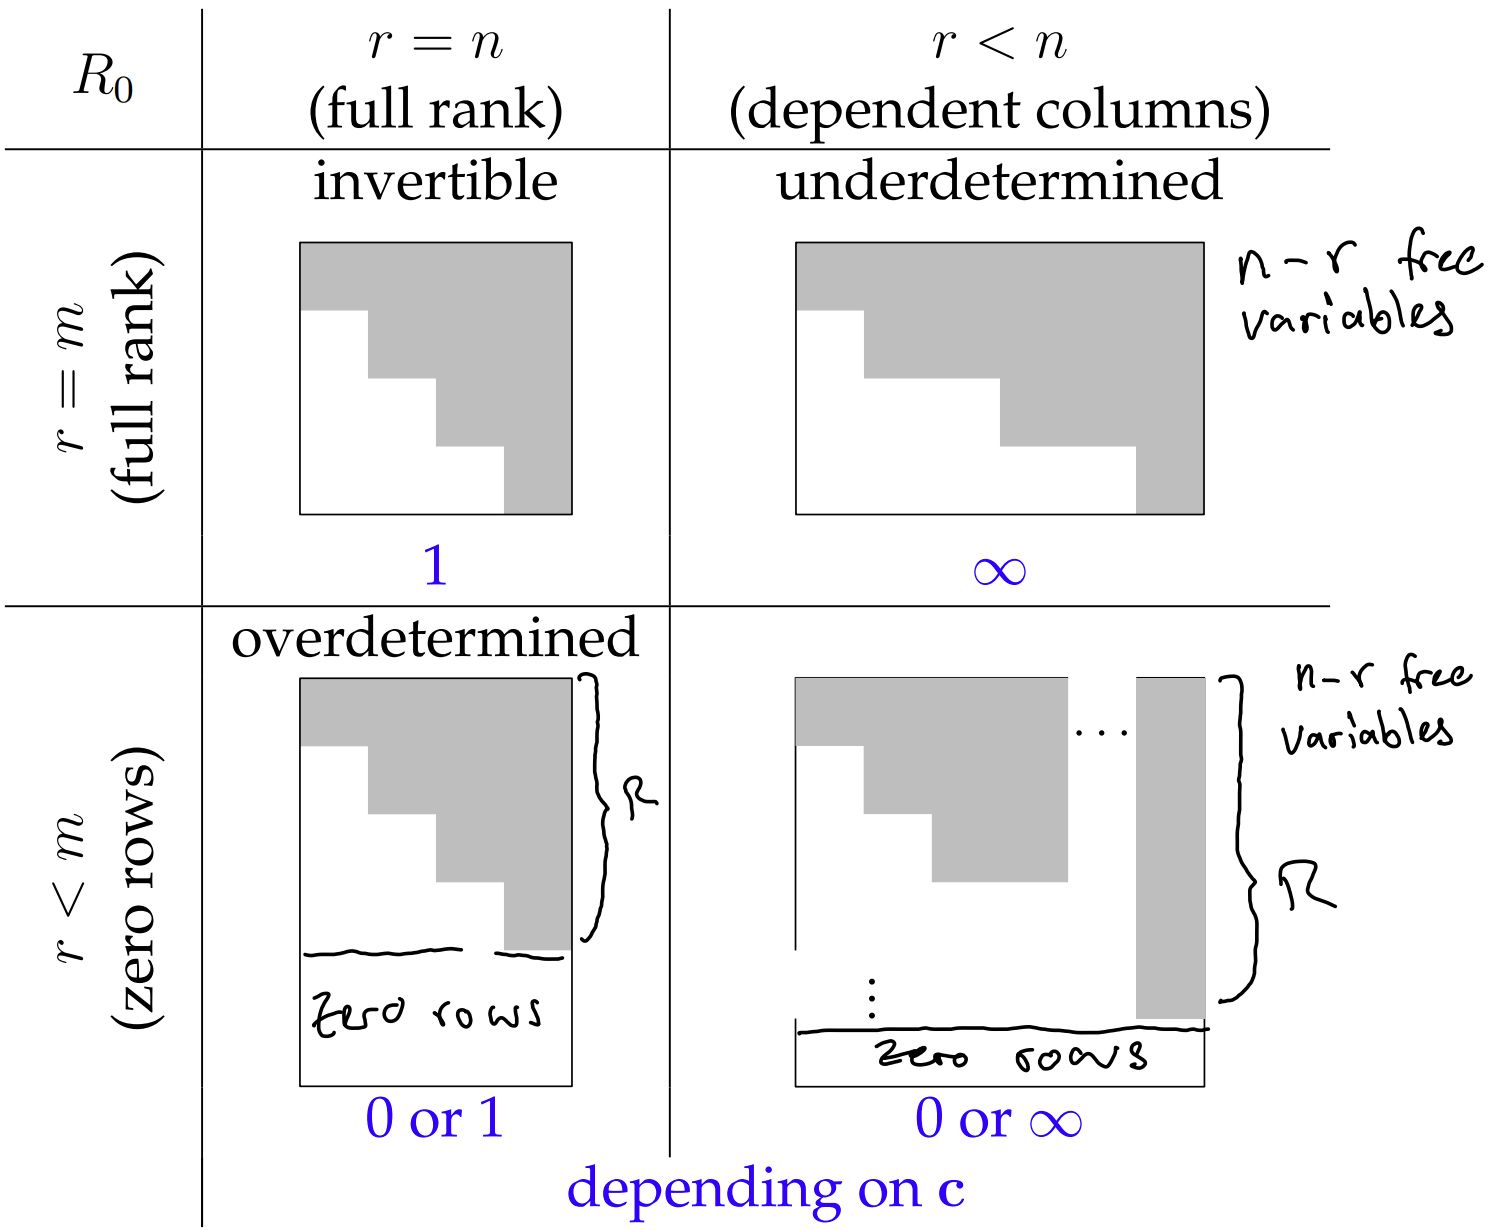
\includegraphics[width=\linewidth,keepaspectratio]{pictures/number_of_solutions.png} 
\end{figure}
Fall 1: all $*=0 \Rightarrow 1, \infty$ solutions.\\
Fall 2: some $*\not=0 \Rightarrow 0$ solutions.

\mysubsection{Basis and Dimension}
\DEF{Basis}{An independent set of vectors that span a vectorspace. Examples:
\begin{enumerate}[nolistsep]
    \item $\{e_1, e_2, ..., e_n\}$ is standard basis of $\mathbb{R}^n$
    \item columns of any invertible $(n\times n)$ matrix are basis of $\mathbb{R}^n$
\end{enumerate}}

\DEF{dimension}{ Let $V$ be a vectorspace. Every basis of $V$ has the same number of vectors. This number is the dimension $dim(V)$ of $V$.
\begin{enumerate}[nolistsep]
    \item $dim(\mathbb{R}^n)=n$
    \item $dim(\begin{bmatrix}
        a & b\\
        c & d
    \end{bmatrix})=4$
    \item $dim(\begin{bmatrix}
        a & 0\\
        0 & d
    \end{bmatrix})=2$ (basis: \begin{bmatrix}
        1 & 0\\
        0 & 0
    \end{bmatrix},
    \begin{bmatrix}
        0 & 0\\
        0 & 1
    \end{bmatrix})
    \item $dim(\begin{bmatrix}
        a & b\\
        b & d
    \end{bmatrix})=3$\\ (basis: $\begin{bmatrix}
        1 & 0\\
        0 & 0
    \end{bmatrix},
    \begin{bmatrix}
        0 & 0\\
        1 & 0
    \end{bmatrix} + \begin{bmatrix}
        0 & 1\\
        0 & 0
    \end{bmatrix},
    \begin{bmatrix}
        0 & 0\\
        0 & 1
    \end{bmatrix}$)
    \item $dim(\{\bm{0}\})=0$ (basis: $\emptyset \rightarrow \bm{0}$ is a combintion of nothing)
\end{enumerate}}

\SA{}{Let $S_n$ be the set of symmetric $n\times n$ matrices which is a subspace of $R^{n\times n}$. Then $dim(S_n)=\begin{cases}
    1 & \text{if $n=1$}\\
    dim(S_{n-1}) + n & \text{else}
\end{cases}=$\\
$ = 1+2+...+n = \frac{n(n+1)}{2}$}


\mysubsection{Orthogonality of Subspaces}
\DEF{}{Two subspaces $V$ and $W$ are orthogonal $\Leftrightarrow v^Tw=0 $ $\forall v\in V, w\in W \Leftrightarrow V \cap W = \{\bm{0}\}$. Let $A$ be $(m\times n)$.
\begin{enumerate}[nolistsep]
    \item $N(A)$ and $C(A^T)$ are orthogonal in $\mathbb{R}^n$
    \item $N(A^T)$ and $C(A)$ are orhogonal in $\mathbb{R}^m$
\end{enumerate}}

\SA{}{Let $V$, $W$ be orthogonal subspaces of $\mathbb{R}^n$. Then $dim(V)+dim(W)\leq n$.}

\DEF{Orthogonal Complement $V^{\perp}$}{Let $V$ be a subspace of $\mathbb{R}^n$. Then $V^{\perp}=\{x\in\mathbb{R}^n|x^Tv=0$ $\forall v\in V\} =$ all vectors in $\mathbb{R}^n$ that are orthogonal to $V$.}

\SA{}{$V^{\perp}$ is a subspace.}

\SA{}{Let $V,W$ be orthogonal complments of $\mathbb{R}^n$. Then $W=V^{\perp} \Leftrightarrow W^{\perp}=V \Leftrightarrow dim(V)+dim(W)=n \Leftrightarrow$ every $u\in \mathbb{R}^n$ can be written as $u=v+w$ with unique vectors $v\in V, w\in W$.}

\mysubsection{The Big Picture}
\hspace{1px}
\begin{figure}[H]
 \centering
 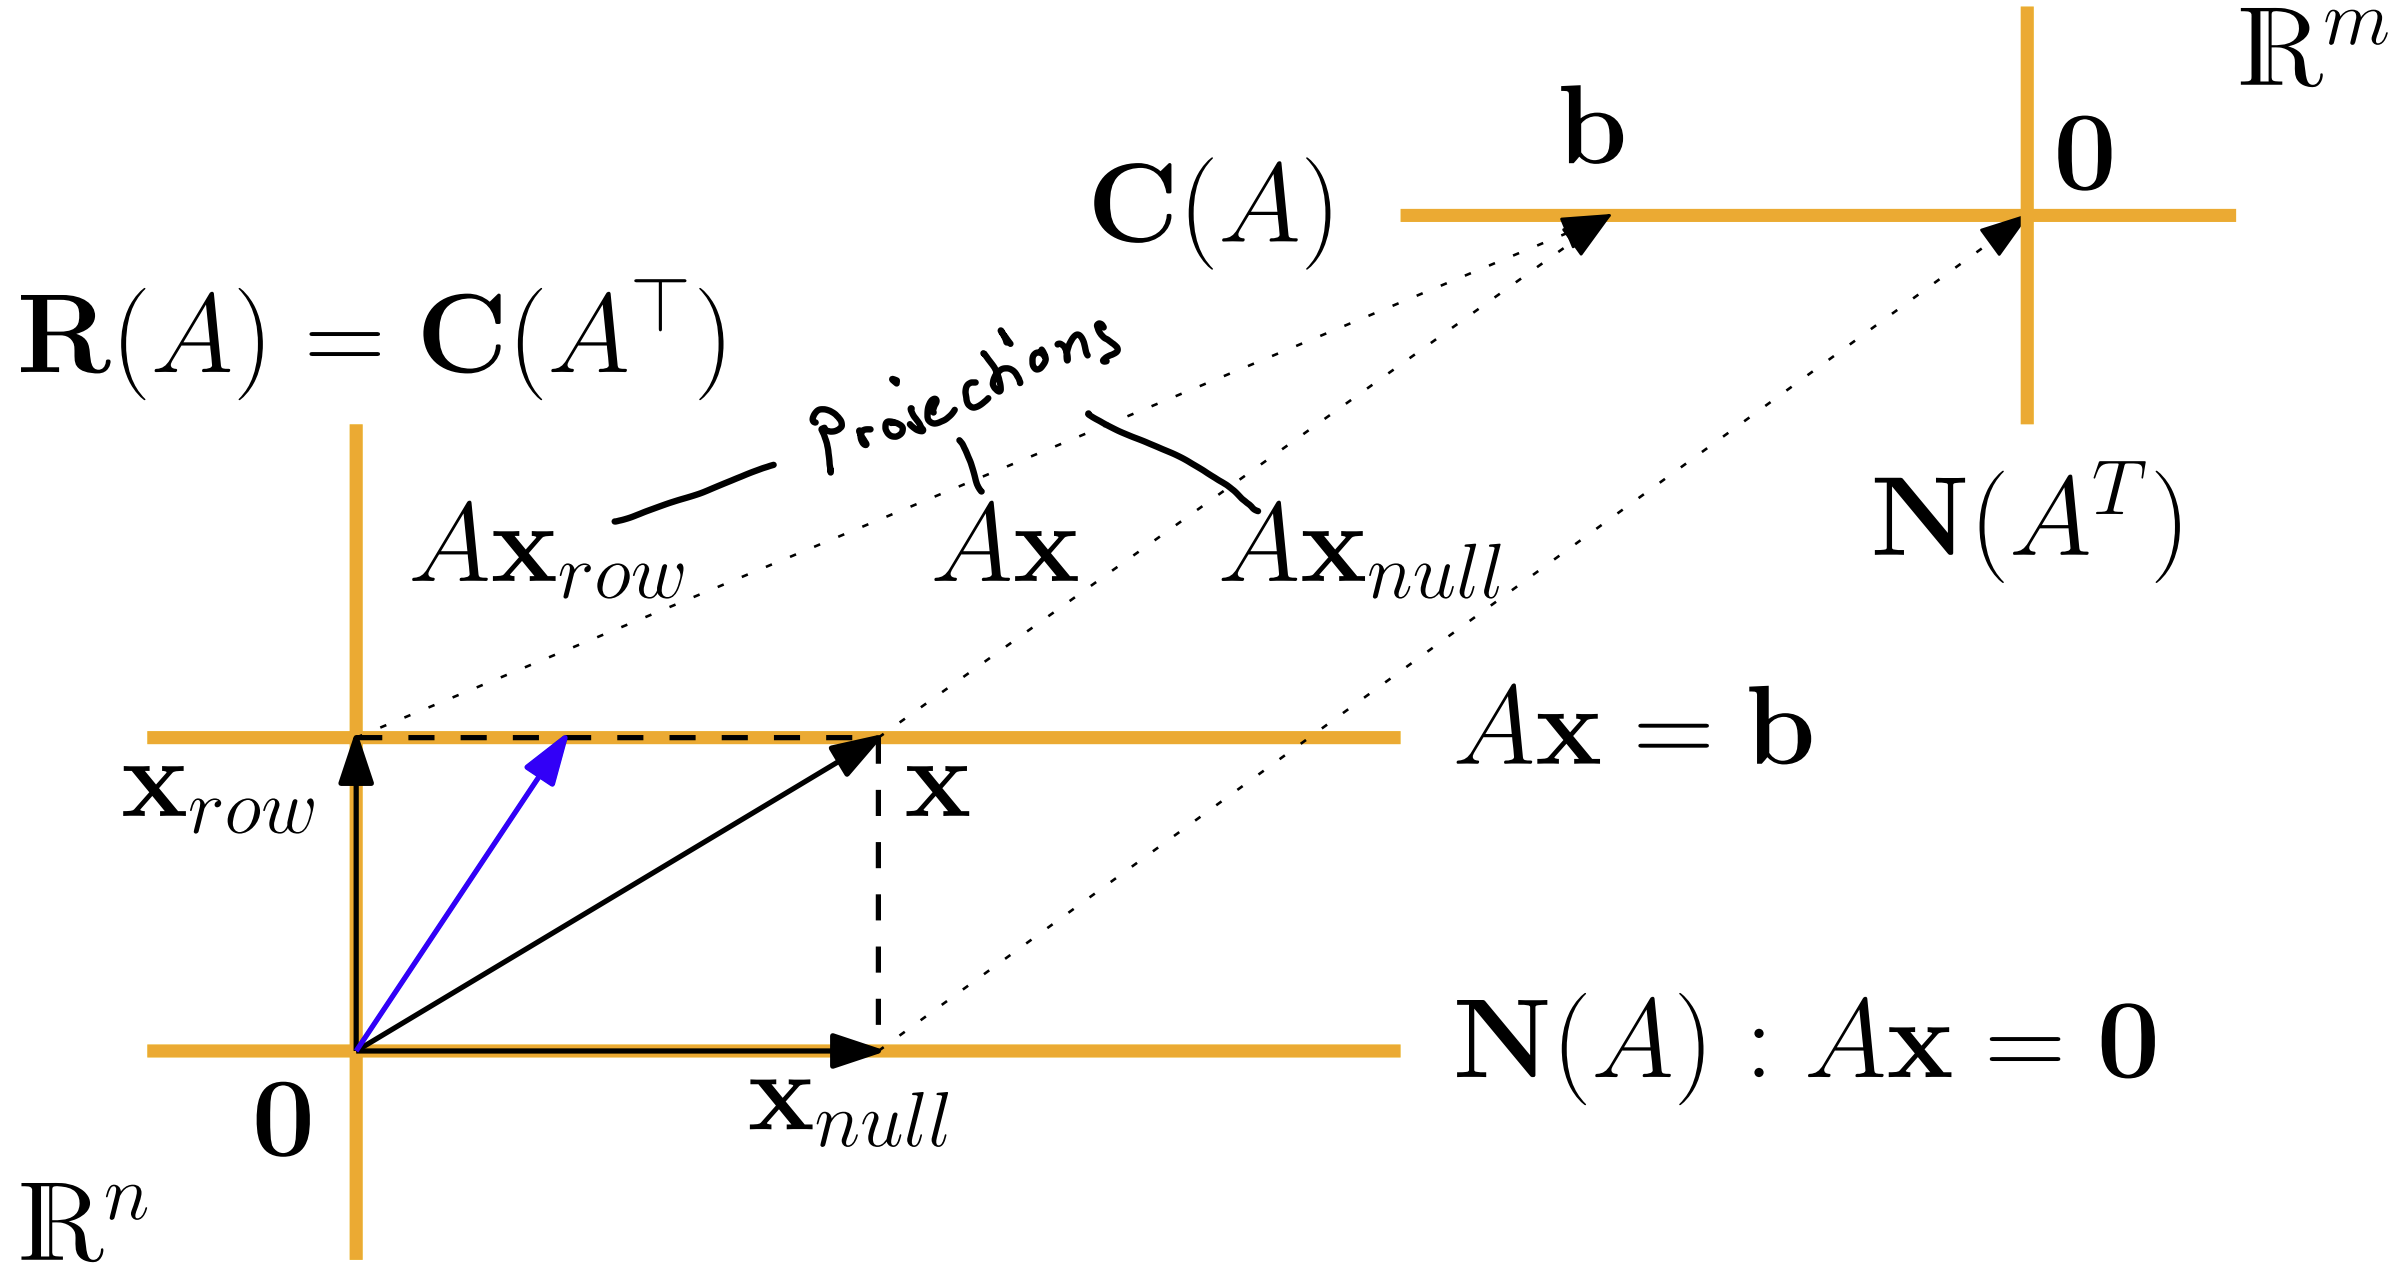
\includegraphics[width=\linewidth,keepaspectratio]{pictures/the_big_picture.png} 
\end{figure}

(solutions of $Ax=b$) $=$ (\color{blue}particular solution \color{black}of $Ax=b$ + solutions of $Ax=\bm{0}$). $N(A)$ and $C(A^T)$, $N(A^T)$ and $C(A)$ are orthogonal subspaces and orthogonal complements. For $x\in\mathbb{R}^n: x=x_{row}+x_{null}$ (row space and nullspace components). If $Ax=b$, then $Ax_{row}=b, Ax_{null}=\bm{0}$.




\mysection[OrangeRed]{\centering Projections and Least Squares}
\DEF{Projection of a vector onto a subspace}{Projection of $b \in \mathbb{R}^m$ onto subspace $S$ of $\mathbb{R}^m$ is the point closest to $b$: $proj_S(b)=\underset{p\in S}{argmin}||b-p||$.}

\COL{Projection onto a line}{Let $a\in \mathbb{R}^m$ non-zero. Let $\hat{x}$ be a scalar s.t. $\hat{x}a = p$. The projection of $b \in \mathbb{R}^m$ on $S=span(a)$ is given by $a^T(b-p)=0 \Leftrightarrow a^T(b-\hat{x}a)=0 \Leftrightarrow proj_S(b)=p=\hat{x}a=Pb=\frac{aa^T}{a^Ta}b$.\begin{itemize}
    \item $b\in span(a) \Leftrightarrow proj_S(b)=b \Leftrightarrow P^2=P$
\end{itemize}}

\COL{Projection onto a subspace}{The projection $p$ of a vector $b\in\mathbb{R}^m$ on a subspace $S$ with basis $a_1, a_2, ..., a_n$ can be written as $p=A\hat{x}$ where $\hat{x}\in\mathbb{R}^n$ satisfies the normal equations: $A^T(b-A\hat{x})=0 \Leftrightarrow A^TA\hat{x}=A^Tb \Leftrightarrow proj_S(b)=p=A\hat{x}=Pb=A(A^TA)^{-1}A^Tb$. Where $A=\begin{bmatrix}
    | & & |\\
    a_1 & \cdots & a_n\\
    | & & |
\end{bmatrix}$. We call $P$ the projection matrix.}

\COL{Projection with Orthonormal Basis}{Let $S$ be subspace of $\mathbb{R}^m$ and $q_1,...,q_n$ orthonormal basis for $S$. Let $Q=\begin{bmatrix}
    q_1, \cdots, q_n
\end{bmatrix}$ be $(m\times n)$. Then projection matrix that projects to $S$ is $P=QQ^T$ and least squares solution to $Qx=b \Leftrightarrow \hat{x}=Q^Tb$.}

\COL{Properties of Projections}
\begin{enumerate}[nolistsep]
    \item $P = P^T \Leftrightarrow P$ is symmetric.
    \item $C(P)=C(A)$
    \item $N(P)=C(A)^{\perp}=C(I-P)$
    
\end{enumerate}




\mysubsection{Linear Regression}
Fit a line through data points $(t_1,b_1),(t_2,b_2),...,(t_m,b_m)$. Find $\alpha_0\in \mathbb{R}$ and $\alpha_1\in\mathbb{R}$ s.t. $b_k\approx\alpha_0+\alpha_1t_k$. Thus $\underset{\alpha_0,\alpha_1}{min}\sum_{k=1}^m(b_k-(\alpha_0+\alpha_1t_k))^2 = \underset{\alpha_0,\alpha_1}{min}||b-A\begin{bmatrix}
    \alpha_0\\
    \alpha_1
\end{bmatrix}||^2 \Leftrightarrow \begin{bmatrix}
    \alpha_0\\
    \alpha_1
\end{bmatrix} = (A^TA)^{-1}A^Tb = \begin{bmatrix}
    m & \sum_{k=1}^mt_k\\
    \sum_{k=1}^mt_k & \sum_{k=1}^mt_k^2
\end{bmatrix}^{-1}\begin{bmatrix}
    \sum_{k=1}^mb_k\\
    \sum_{k=1}^mt_kb_k
\end{bmatrix}$ this equals to $\begin{bmatrix}
    \frac{1}{m}\sum_{k=1}^mb_k\\
    (\sum_{k=1}^mt_kb_k) / (\sum_{k=1}^mt_k^2)
\end{bmatrix}$ if $A^TA$ is diagonal. Where $b=\begin{bmatrix}
    b_1\\
    \vdots\\
    b_m
\end{bmatrix}$ and $A=\begin{bmatrix}
    1 & t_1\\
    \vdots & \vdots\\
    1 & t_m
\end{bmatrix}$.

If $A^TA$ not diagonal, we have $\begin{bmatrix}
    \alpha_0\\
    \alpha_1
\end{bmatrix} = \begin{bmatrix}
    \frac{1}{m}\sum_{k=1}^mb_k\\
    (\sum_{k=1}^mt'_kb_k) / (\sum_{k=1}^mt'_k^2)
\end{bmatrix} + \begin{bmatrix}
    c(\sum_{k=1}^mt'_kb_k) / (\sum_{k=1}^mt'_k^2)\\
    0
\end{bmatrix}$ with $t'_k = t_k+c$ and $c=-\frac{1}{m}\sum_{k=1}^mt_k$.




\mysubsection{Gram-Schmidt Algorithm}
Given $n$ linearly independent vectors $a_1,...,a_n$ that span a subspace $S$, the Gram-Schmidt process constructs the orthonormal basis $q_1,...,q_n$ the following way:
\begin{itemize}
    \item $q_1=\frac{a_1}{||a_1||}$
    \item For $k=2,...,n$ do\\
    \hspace{1.8em}$q_k'=a_k-\sum_{i=1}^{k-1}(a_k^Tq_i)q_i$\\
    \hspace{1.8em}$q_k=\frac{q_k'}{||q_k'||}$
\end{itemize}
$q_k' = a_k -$ (projection of $a_k$ onto the subspace spanned by the $k$ vectors before it).

\SA{}{Every vector space ($\not=\infty$) has an orthonormal basis.}

\COL{A=QR Decomposition}
Let $A$ be $m\times n$ with linearly independent columns. Then $A=QR \Leftrightarrow R=Q^TA$ where Q is $m\times n$ with orthonormal columns (output of Gram-Schmidt on columns of $A$). $R$ is $n\times n$ and upper triangular.
\begin{enumerate}[nolistsep]
    \item $rank(A)=n \Leftrightarrow N(A)=\{\bm{0}\} \Leftrightarrow N(R)=\{\bm{0}\} \Leftrightarrow R, R^T$ invertible.
    \item $C(A)=C(Q) \Leftrightarrow proj_{C(A)}(b)=QQ^Tb$
    \item Since $A^TA=(QR)^T(QR)=R^TQ^TQR=R^TR$ we have for the least squares solution that $A^TA\hat{x}=A^Tb \Leftrightarrow R^TR\hat{x}=R^TQ^Tb \Leftrightarrow R\hat{x}=Q^Tb$.
\end{enumerate} 




\mysubsection{Pseudoinverse}
\DEF{Pseudoinverse (Moore-Penrose Inverse)}{
\color{OrangeRed}If $rank(A)=n$ \color{Black} For $A\in\mathbb{R}^{m\times n}$ we define the pseudo-inverse $A^\dag\in\mathbb{R}^{n\times m}$ of $A$ as $A^\dag=(A^TA)^{-1}A^T$ which is a left inverse: $A^\dag A=I$.\\
\color{OrangeRed}If $rank(A)=m$ \color{Black} $A^\dag=A^T(AA^T)^{-1}$ which is a right-inverse: $AA^\dag=I$. Further the unique solution to $min_{x\in\mathbb{R}^n}||x||^2$ s.t. $Ax=b$ is given by $\hat{x}\in C(A^T)$ s.t. $A\hat{x}=b \Leftrightarrow \hat{x}=A^{\dag}b$.\\
\color{OrangeRed}For all matrices \color{black} $A^\dag=R^\dag C^\dag=R^T(RR^T)^{-1}(C^TC)^{-1}C^T=R^T(C^TCRR^T)^{-1}C^T=R^T(C^TAR^T)^{-1}C^T$. This also works for any other decomposition of $A$ as long as the resulting matrices have either full row-rank or full column-rank.}

\SA{Calculation Rules}{Let $A\in\mathbb{R}^{m\times n}$ and $B\in\mathbb{R}^{n\times p}$. Then
\begin{enumerate}[nolistsep]
    \item $(AB)^\dag=B^\dag A^\dag$, as long as $rank(A)=rank(b)=n$.
    \item $(A^T)^\dag=(A^\dag)^T$.
    \item $AA^\dag$ is symmetric, and is the projection matrix for projection on $C(A)$.
    \item $A^\dag A$ is symmetric, and is the projection matrix for projection on $C(A^T)$.
    \item $rank(A) = rank(A^\dag)$.
\end{enumerate}}




\mysection[Aquamarine]{\centering Linear Transformations}
\SA{}{$A:x\rightarrow Ax$ can be viewed as a function from $C(A^T)$ to $C(A)$. It is a bijection. Hence $\forall$ $b\in C(A)$ $\exists$ unique $x\in C(A^T)$ s.t. $Ax=b$.}

\SA{}{Given two vector spaces $U, V$, a Linear Transformation is a function $T:U\rightarrow V$ s.t. $\forall u_1,u_2\in U$ and $\alpha \in \mathbb{R}$ the following 2 properties hold
\begin{enumerate}[nolistsep]
    \item $T(u_1+u_2)=Tu_1 + Tu_2$
    \item $T(\alpha u_1)=\alpha Tu_1$
\end{enumerate}}
Hence also $T(\alpha_1u_1+...+\alpha_ku_k)=\alpha_1T(u_1)+...+\alpha_kT(u_k)$.

\SA{}{Let $T:U\rightarrow V$ and $L:U\rightarrow V$ that take the same value in a basis $u_1,...,u_n$ of $U$. Then $T=L$.}

\SA{}{Given basis $u_1,...,u_n$ of $U$, and any $v_1,...,v_n \in V$ there is a linear transformation $T:U\rightarrow V$ s.t. $\forall 1\leq i \leq n, T(u_i)=v_i$.}

\SA{}{For any Linear Transformation $T:\mathbb{R}^n\rightarrow\mathbb{R}^m$, there exists an $m\times n$ matrix A s.t. $T(x)=Ax$ $\forall x\in\mathbb{R}^n$.}

\SA{}{Let $T:\mathbb{R}^n\rightarrow \mathbb{R}^m$ and $L:\mathbb{R}^m\rightarrow\mathbb{R}^p$, with corresponding matrices $A, B$. Then $L\circ T(x)=L(T(x))=BAx$}

\COL{Examples}}
\begin{enumerate}[nolistsep]
    \item Stretch: y-axis by factor 2 $A=\begin{bmatrix}
        1 & 0\\
        0 & 2
    \end{bmatrix}$
    \item Shear: $A=\begin{bmatrix}
        1 & 0\\
        1 & 1
    \end{bmatrix}$
    \item Rotation: $A=\begin{bmatrix}
        \frac{1}{\sqrt{2}} & -\frac{1}{\sqrt{2}}\\
        \frac{1}{\sqrt{2}} & \frac{1}{\sqrt{2}}
    \end{bmatrix}$ counterclockwise by $45^{\circ}=\frac{\pi}{4}$.
    \item Reflection: $A=\begin{bmatrix}
        0 & 1\\
        1 & 0
    \end{bmatrix}$ by the diagonal line $x_2=x_1$
    \item Reflection: Let $v\in\mathbb{R}^n$ s.t. $||v||=1$. Then $A=I-2vv^T$ reflects along the hyperplane $H=\{x\in\mathbb{R}^n|x^Tv=0\}$.
\end{enumerate}


\mysubsection{Change of Basis}
\COL{Canonical Basis}Let $A^{n\times m}$ represent a linear transformation $L:\mathbb{R}^n\rightarrow\mathbb{R}^m$ given by $x\in\mathbb{R}^n \rightarrow Ax\in\mathbb{R}^m$. We can write in- and output in the canonical bases as $x=\sum_{j=1}^nx_je_j$ and $Ax=\sum_{i=1}^m(Ax)_ie_i$.

\COL{Arbitrary Basis}Let $u_1,...,u_n$ be a basis for $\mathbb{R}^n$ and $v_1,...,v_n$ for $\mathbb{R}^m$. Let $U\in\mathbb{R}^{n\times n}$ have $u_1,...,u_n$ and $V\in\mathbb{R}^{m\times m}$ have $v_1,...,v_n$ as columns. Then $L$ takes a vector $x=\sum_{j=1}^n\alpha_ju_j=U\alpha$ and outputs $L(x)=AU\alpha=\sum_{i=1}^m\beta_iv_i=V\beta \Leftrightarrow \beta=V^{-1}AU\alpha = B\alpha \Leftrightarrow B=V^{-1}AU$ where $\alpha\in\mathbb{R}^n$ and $\beta\in\mathbb{R}^m$.

\mysubsection{Diagonalization}
\DEF{Eigendecomposition}{Let $A\in\mathbb{R}^{n\times n}$ with a complete set of real eigenvectors. Let $v_1,...,v_n\in\mathbb{R}^{n}$ be a basis formed with eigenvectors of $A$. Let $\lambda_1,...,\lambda_n$ be the associated eigenvalues. Let $V\in\mathbb{R}^{n\times n}$ be the matrix with $v_1,...,v_n$ as columns. Then $A=V\Lambda V^{-1} \Leftrightarrow \Lambda=V^{-1}AV$, where $\Lambda$ is a diagonal matrix with $\Lambda{ii}=\lambda_i$.}

\RC{Eigendecomposition}{\begin{enumerate}[nolistsep]
    \item find the eigenvalues of $A$ $\lambda_k$ and write $\Lambda = diag(\lambda_1 \cdots \lambda_n)$
    \item find the according eigenvectors $v_k $ of  $\lambda_k$ write  them as $V = (v_1|\cdots|v_n) $ (sorted according to $\Lambda $) 
    \item find inverse $V^T=V^{-1}$
\end{enumerate}}


\DEF{Diagonalizable}{Let $A\in\mathbb{R}^{n\times n}$. $\exists V^{-1}$ s.t. $\Lambda=V^{-1}AV \Leftrightarrow A$ is diagonalizable.}

\DEF{Similar Matrices}{We say $A\in\mathbb{R}^{n\times n}$ and $B\in\mathbb{R}^{n\times n}$ are similar if $\exists$ invertible matrix $S$ s.t. $B=S^{-1}AS$.}

\SA{}{Let $B=S^{-1}AS \Leftrightarrow A,B$ similar. Then \begin{enumerate}[nolistsep]
    \item $tr(A)=tr(B)$
    \item $det(A)=det(B)$
    \item $A,B$ have the same eigenvalues
\end{enumerate}}





\mysection[Orchid]{\centering Determinants}
\DEF{}{$det(a) = a, det\begin{pmatrix}
a & b  \\
c & d \\
\end{pmatrix}=\begin{vmatrix}
 a & b\\
 c & d
\end{vmatrix} = ad-bc$,\\
$det\begin{pmatrix}
a & b & c  \\
d & e & f \\
 g & h & i  \\
\end{pmatrix} = aei+bfg+cdh-ceg-bdi-afh = a\begin{vmatrix}
    e&f\\
    h&i
\end{vmatrix}-b\begin{vmatrix}
    d & f\\
    g & i
\end{vmatrix}+c\begin{vmatrix}
    d & e\\
    g & h
\end{vmatrix}=\sum_{j=1}^nA_{i,j}C_{i,j}$}

\DEF{}{$det(A) = 0 \Leftrightarrow A $ is singular $\Leftrightarrow \not\exists A^{-1}$}

\DEF{}{$det(A) \neq 0 \Leftrightarrow A $ is regular $\Leftrightarrow \exists A^{-1}$}

\DEF{Sign of Permutation}{Given permutation $\sigma:\{1,...,n\}\rightarrow\{1,...,n\} \Leftrightarrow \sigma: x \rightarrow Px$, then $sgn(\sigma)$ can be 1 or -1. The sign counts the parity of the number of pairs of elements that are out of order (sometimes called inversions) after applying the permutation.
Let $(i,j)\in\{1,...,n\}\times\{1,...,n\}$. Then $sgn(\sigma)=$
\begin{cases}
    1 & \text{if $|i < j \land \sigma(i)>\sigma(j)|$ is even}\\
    -1 & \text{if $|i < j \land \sigma(i)>\sigma(j)|$ is odd}
\end{cases}}

\DEF{}{Given square matrix $A\in\mathbb{R}^{n\times n}$. Then $det(A)=\sum_{\sigma\in\prod_n}sgn(n)\prod_{i=1}^nA_{i,\sigma(i)}$. Where $\prod_n$ is the set of all permutations of $n$ elements.}

\SA{}{Given permutation matrix $P\in\mathbb{R}^{n\times n}$ corresponding to a permutation $\sigma$. Then $det(P)=sgn(\sigma)=sgn(P)$.}

\SA{}{Let $A,B\in\mathbb{R}^{n\times n}$. Then $det(AB)=det(A)det(B)$.}

\SA{}{Let $T\in\mathbb{R}^{n\times n}$ triangular. Then $det(T)=\prod_{k=1}^nT_{kk}$.}

\SA{}{Let $A\in\mathbb{R}^{n\times n}$. Then $det(A^T)=det(A)$.}

\SA{}{Let $Q\in\mathbb{R}^{n\times n}$ be orthogonal. Then $det(Q) = \pm1$.}

\SA{}{Let $A\in\mathbb{R}^{n\times n}$ and $det(A)\not=0$. Then $det(A^{-1})=\frac{1}{det(A)}$.}

\DEF{}{Let $A\in\mathbb{R}^{n\times n}$. Then $\mathscr{A}_{i,j}$ denotes the $(n-1)\times(n-1)$ matrix obtained by removing row $i$ and column $j$ from $A$.}

\DEF{Co-factors of A}{Let $A\in\mathbb{R}^{n\times n}$. Then $C_{i,j}=(-1)^{i+j}det(\mathscr{A}_{i,j}) \Rightarrow det(A)=\sum_{j=1}^nA_{i,j}C_{i,j}$ with $1 \leq i \leq n$.}

\SA{}{Let $A\in\mathbb{R}^{n\times n}$ with $det(A)\neq0$. Then $A^{-1}=\frac{1}{det(A)}C^T \Leftrightarrow AC^T=det(A)I$ where $C$ is $(n\times n)$ with the co-factors of $A$ as entries.}

\DEF{Cramer's Rule}{Let $A\in\mathbb{R}^{n\times n}$ with $det(A)\neq0$ and $b\in\mathbb{R}^n$. Then the solution $x\in\mathbb{R}^n$ of $Ax=b$ is given by $x_j=\frac{det(\mathscr{B}_j)}{det(A)}$ where $\mathscr{B}_j$ is the matrix obtained by $A$ by replacing column $j$ of $A$ with $b$.}

\DEF{Efficient calculation of Determinant}{$PA=LU \Rightarrow det(P)=sgn(P), det(L)=1 \Rightarrow det(A)=\frac{1}{det(P)}det(L)det(U)=sgn(P)det(U)$.}

\SA{}{If $A$ is $(n\times n)$ and $P$ is permutation that swaps two rows of $A$ then $det(PA)=-det(A)$.}


\SA{}{\begin{enumerate}[nolistsep]
\item if A has a row with 0 $\Rightarrow det(A)=0$
\item multiplying a row with a factor increases the determinant by the same factor. Hence $det(\gamma A) = \gamma^n det(A)$.
\item if A has to equal rows  $\Rightarrow det(A)=0$
\item adding a multiple of a row to another row doesn't affect the det
\end{enumerate}
Every statement also holds for columns instead of rows.}

\DEF{det of block matrices}{$det \left[ 
\begin{array}{c|c} 
  A & C \\ 
  \hline 
  0 & B
\end{array} 
\right]  = det (A)\cdot det(B)$}




\mysection[BrickRed]{\centering Complex Numbers}
\mysubsection{Basics}
\DEF{}{$\mathbb{C}=\{a+ib|a,b\in\mathbb{R}, i^2=-1\}$.}

\DEF{}{$z = a + ib \Leftrightarrow \Re (z)=a, Im(z)=b $}

\SA{Operations}{\begin{enumerate}[nolistsep]
    \item $(a+ib)+(x+iy)=(a+x)+i(b+y)$
    \item $(a+ib)(x+iy)=ax+i(ay+bx)+i^2by=ax+i(ay+bx)-by=(ax-by)+i(ay+bx)$
    \item $(a+ib)(a-ib)=a^2+b^2$
    \item $\frac{a+ib}{x+iy}=\frac{(x-iy)(a+ib)}{(x-iy)(x+iy)}=\frac{(ax+by)+i(bx-ay)}{x^2+y^2}=(\frac{ax+by}{x^2+y^2})+i(\frac{bx-ay}{x^2+y^2})$
    \item $|z|=|a+ib|=\sqrt{a^2+b^2}$
    \item $\overline{a+ib}=a-ib$
    \item $|z|^2=z\overline{z}$
    \item Let $z_1,z_2\in\mathbb{C}$. Then
    \item[8a] $z_1z_2=z_2z_1$
    \item[8b] $\overline{z_1+z_2}=\overline{z_1}+\overline{z_2}$
    \item[8c] $\frac{1}{z}=\frac{\overline{z}}{|z|^2}$
\end{enumerate}}

\DEF{Euler's Formula}{Let $\theta\in\mathbb{R}$. Then $e^{i\theta}=cos\theta+isin\theta \Leftrightarrow e^{i\pi}=-1 \Leftrightarrow e^{i\pi}+1=0$.}

\DEF{Polar Coordinates}{Let $z\in\mathbb{C}$. Then $z=re^{i\theta}$ where $r\geq0$ is the modulus of $z$ and $\theta\in[0,2\pi]$ is an angle, also called the argument of $z$.}

\DEF{Fundamental Theorem of Algebra}{For any degree $n$ non-constant ($n\geq1$) polynomial $P(z)=\alpha_nz^n+a_{n-1}z^{n-1}+...+\alpha_1z+\alpha_0$ with $a_n\neq0$ $\exists \lambda\in\mathbb{C}$ s.t. $P(\lambda)=0 \Rightarrow \mathbb{C}$ is algebraically closed.}

\SA{Characteristics Polynomial}{Any degree $n$ non-constant ($n\geq1$) polynomial $P(z)=\alpha_nz^n+a_{n-1}z^{n-1}+...+\alpha_1z+\alpha_0$ with $\alpha_n\neq0$ has $n$ zeros: $\lambda_1,...,\lambda_n\in\mathbb{C}$, perhaps with repetitions, s.t. $P(z)=\alpha_n(z-\lambda_1)(z-\lambda_2)...(z-\lambda_n)$. This is called the characteristics polynomial. The number of times $\lambda\in\mathbb{C}$ appears in this expansion is called the algebraic multiplicity of the zero.}

\DEF{Hermetian Transpose}{Also called conjugate transpose. Is the natural operation of transposing for complex vectors and matrices: $A^*=\overline{A}^T=A^H$.}

\begin{figure}[H]
 \centering
 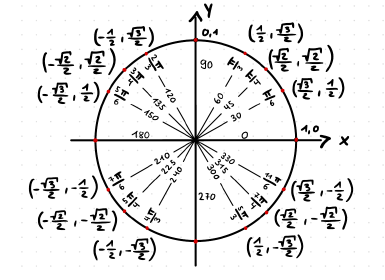
\includegraphics[width=\linewidth,keepaspectratio]{pictures/complex_numbers.png}
\end{figure}





\mysection[Magenta]{\centering Eigenvalues and -vectors}
\DEF{Quadratic Formula}{$ax^2+bx+c=0 \Rightarrow x=\frac{-b\pm\sqrt{b^2-4ac}}{2a}$.}

\DEF{}{Let $A\in\mathbb{R}^{n\times n}$. Then $\lambda\in\mathbb{C}$ is an eigenvalue of $A$ and $v\in\mathbb{C}^n-\{\bm{0}\}$ is a corresponding eigenvector of $A$ iff $Av=\lambda v \Leftrightarrow Av-\lambda v = (A-\lambda I)v = 0 \Leftrightarrow det(A-\lambda I)=0 \Rightarrow \exists v\in N(A-\lambda I) - \{0\}$.}

\SA{}{$det(A-\lambda I)$ is a polynomial in $\lambda$ of degree $n$. The coefficient of the $\lambda^n$ is $(-1)^n$.}

\SA{}{The fundamental theorem of algebra implies that every matrix $A\in\mathbb{R}^{n\times n}$ has an eigenvalue (perhaps $\in\mathbb{C}$).}

\SA{}{Let $M\in\mathbb{R}^{n\times n}$ and $c\in\mathbb{R}$. Then $\forall$ real eigenvalues $\lambda\in\mathbb{R}$ of $M$, $\lambda+c$ is a real eigenvalue of $M+cI$.}

\SA{}{$A^kv=\lambda^kv$ for $k\geq1$.}

\SA{}{Let $A$ be invertible. Then $Av=\lambda v \Leftrightarrow A^{-1}v=\frac{1}{\lambda}v$.}

\SA{}{Let $A^{n\times n}$ and $v_1,...,v_k\in\mathbb{R}^n$ be eigenvectors corresponding to eigenvalues $\lambda_1,...,\lambda_k\in\mathbb{R}^n$. $\lambda_1,...,\lambda_k$ all distinct $\Leftrightarrow v_1,...,v_k$ linearly independent.}

\SA{}{Let $A\in\mathbb{R}^{n\times n}$ with $n$ real distinct eigenvalues then there is a basis of $v_1,...,v_n$ of $\mathbb{R}^n$ made up of eigenvectors of $A$.}

\SA{}{Let $A\in\mathbb{R}^{n\times n}$. Then $det(A-zI)=det((A-zI)^T)=det(A^T-zI) \Leftrightarrow$ $A$ and $A^T$ share the same eigenvalues.}

\DEF{Trace}{$Tr(A)=\sum_{i=1}^nA_{ii}=\sum_{i=1}^n\lambda_i$ and $det(A)=\prod_{i=1}^n\lambda_i$.}

\SA{}{Let $Q\in\mathbb{R}^{n\times n}$ be orthogonal. If $\lambda\in\mathbb{C}$ is an eigenvalue of $Q$, then $|\lambda|=1$.}

\DEF{Complete Set of Real Eigenvectors}{Given $A\in\mathbb{R}^{n\times n}$. $A$ has a complete set of real eigenvectors $\Leftrightarrow$ we can build a basis of $R^n$ with real eigenvectors of $A \Leftrightarrow$ geometric multiplicities are the same as the algebraic multiplicities for all eigenvalues.}

\SA{}{Let $P$ be the projection matrix on the subspace $U\subseteq\mathbb{R}^n$. Then $P$ has two eigenvalues, $0$ and $1$, and a complete set of real eigenvectors.}

\DEF{Geometric Multiplicity}{Given $A\in\mathbb{R}^{n\times n}$ and an eigenvalue $\lambda$ of $A$ we call the dimension of $N(A-\lambda I)$ the geometric multiplicity of $\lambda$.}

\DEF{Algebraic Multiplicity}{The  multiplicity of an eigenvalue in the char. polynomial.}

\SA{}{Geometric multiplicity $\leq $ algebraic multiplicity. If $A$ symmetric then always equal.}

\SA{Words of Caution}{\begin{enumerate}[nolistsep]
    \item Eigenvalues of $A$ and $A^T$ are the same, the eigenvectors NOT!
    \item The eigenvalues of $A+B$ are not easily computed from the eigenvalues of $A$ and $B$, in particular they are not their sum!
    \item The eigenvalues of $AB$ or $BA$ are not easily computed from the eigenvalues of $A$ and the ones of $B$, in particular they are not their product!
    \item Gaussian Elimination doesn't preserve eigenvalues and eigenvectors. The eigenvalues are not the diagonal elements of the $U$ matrix of $PA=LU$.
\end{enumerate}}

\DEF{Spectral Theorem}{Any $A\in\mathbb{R}^{n\times n}$ that is symmetric has $n$ real eigenvalues and an orthonormal basis of $\mathbb{R}^n$ made of eigenvectors of $A$. Hence $A=V\Lambda V^T=\sum_{k=1}^n\lambda_iv_iv_i^T \Rightarrow rank(A)=$ \# of non-zero eigenvalues of A.}

\SA{}{Every real symmetric matrix has a real eigenvalue $\lambda$.}

\DEF{Rayleigh Quotient}{Given symmetric $A\in\mathbb{R}^{n\times n}$. Then $R:\mathbb{R}^n\setminus\{0\}\rightarrow\mathbb{R}$ where $R(x)=\frac{x^TAx}{x^Tx}$ attains its max at $R(v_{max})=\lambda_{max}$ and its min at $R(v_{min})=\lambda_{min}$ where $\lambda_{max},\lambda_{min}$ are largest and smallest eigenvalues of $A$ and $v_{max},v_{min}$ their associated eigenvectors.}

\DEF{Positive Definite (PD) and Positive Semidefinite (PSD)}{Let $A\in\mathbb{R}^{n\times n}$ symmetric. \begin{itemize}
    \item $A$ is PSD $\Leftrightarrow$ all eigenvalues non-negative $\Leftrightarrow x^TAx\geq0$ $\forall$ $x\in\mathbb{R}^n\setminus\{0\}$.
    \item $A$ is PD $\Leftrightarrow$ all eigenvalues strictly positive $\Leftrightarrow x^TAx>0$ $\forall$ $x\in\mathbb{R}^n\setminus\{0\}$. 
\end{itemize}}

\DEF{Gram Matrix $V^TV$}{Given $v_1,...,v_m\in\mathbb{R}^n$ then $G_{ij}=v_i^Tv_j \Leftrightarrow G=V^TV\in\mathbb{R}^{m\times m}$ where $v_1,...,v_m$ columns of $V\in\mathbb{R}^{n\times m}$.}

\DEF{Gram Matrix $AA^T$}{Given $A\in\mathbb{R}^{m\times n}$. $AA^T=\sum_{i=1}^ma_ia_j^T\in\mathbb{R}^{m\times m}$ where $a_1,...,a_n\in\mathbb{R}^m$ columns of $A$.}

\DEF{Cholesky Decomposition}{Let $M$ be PSD matrix. Then $M=C^TC$ where $C$ is upper-triangular.}

\SA{}{$rank(A)=$\# of non-zero eigenvalues of $A \Rightarrow$ a square matrix is singular $\Leftrightarrow$ it has $0$ as an eigenvalue.}


\mysection[WildStrawberry]{\centering Singular Value Decomposition (SVD)}
SVD generalizes the eigendecomposition to non-symmetric, and even non-square matrices. 

\DEF{SVD}{Let $A\in\mathbb{R}^{m\times n}$. Then $\exists$ orthogonal matrices $U\in\mathbb{R}^{m\times m}$ and $V\in\mathbb{R}^{n\times n}$ s.t. $A=U\Sigma V^T$, where $\Sigma\in\mathbb{R}^{m\times n}$ is a diagonal matrix with non-negative diagonal elements ordered in descending order that are called the singular values of $A$.\\
The columns $u_1,...,u_m$ of $U$ are called left singular vectors of $A$. The columns $v_1,...,v_m$ of $V$ are called right singular vectors of $A$.}

\DEF{SVD with $rank(A)=r$}{$A=U_r\Sigma_rV_r^T=\sum_{k=1}^r\sigma_ku_kv_k^T$ where $U_r\in\mathbb{R}^{m\times r}$ contains the first $r$ left singular vectors, $V_r\in\mathbb{R}^{n\times r}$ the first $r$ right singular vectors, and $\Sigma_r\in\mathbb{R}^{r\times r}$ the first $r$ singular values on its diagonal.}

\SA{}{$AA^T=U(\Sigma\Sigma^T)U^T$. Hence, left singular vectors of $A$ = eigenvectors of $AA^T$.}

\SA{}{$A^TA=V(\Sigma^T\Sigma)V^T$. Hence, right singular vectors of $A$ = eigenvectors of $A^TA$.}

\SA{}{$\Sigma^T\Sigma = \Sigma\Sigma^T = diag(\sigma_1^2,...,\sigma_n^2)$ $ = diag(\lambda_1,...,\lambda_n)$. Hence, the singular values of $A$ = square-root of eigenvalues of $AA^T$ and $A^TA$.}

\SA{}{$rank(A)=$\# of non-zero singular values of $A$.}

\SA{}{Every matrix $A\in\mathbb{R}^{m\times n}$ has an SVD decomposition $\Leftrightarrow$ every linear transformation is diagonal when viewed in the bases of the singular vectors.}





\mysection[WildStrawberry]{\centering Decompositions}

\KRZ{Eigenvaluedecomposition with SVD}{ The SVD is given by $A = U \Sigma V^H$
\begin{itemize}
\item[1]  Expand $U \Sigma V^H \Rightarrow U I \Sigma V^H  \Rightarrow U I_{1} I_{2} \Sigma V^H $ where $U I_{1} = V $ and  $I_{1} I_{2} = I $
\item[2] Calculate $
\left ( U I_{1}  \right ) \left (I_{2} \Sigma  \right ) V^H  $
\end{itemize}} 


\KRZ{Composition of 1-rank- matrices}{
\begin{itemize}
    \item[1] write $A = V \Lambda V^{-1 }$
    \item[2] rewrite $ A = \sum_{k=1}^{n}V_k \lambda_k w_k^T $
    \textit{$V_k $ = row ($\downarrow $) of $V$, $w_k^T $ = column ($\rightarrow $) of $V^{-1}$.}
\end{itemize}}


}

\KRZ{Powers of $A$}{
\begin{itemize}
\item[1] write $A = V \Lambda V^{-1 }$ 
\item[2] calculate $A^m = V \Lambda^m V^{-1 }$
\end{itemize}
note: $\Lambda^m = diag(a_{11}^m , \cdots , a_{nn}^m)$.}

\KRZ{SVD of $A \in \mathbb{E}^{m \times n}$with $A^HA $}{\begin{itemize}
\item[1] Calculate $(A^HA)\in \mathbb{E}^{n \times n}$
\item[2] find eigenvalue of $A^HA$
 \item[3] write $\Sigma_r = diag(\sqrt{\lambda_{1}}, \cdots, \sqrt{\lambda_{n}}) \in \mathbb{E}^{n \times n}$
\item[4] rewrite: $\Sigma \in \mathbb{E}^{m \times n} $: $\Sigma = \begin{smallmatrix}
 \Sigma_r&  0\\
 0& 0 \\
\end{smallmatrix}$
\item[5] find eigenvectors of $A^HA \Rightarrow v_1 ,\cdots ,v_r$
\item[6] norm eigenvectors and compute $V = ( \frac{v_1}{\left\| v_1 \right\|}|\cdots| \frac{v_n}{\left\| v_n \right\|}) \in \mathbb{R}^{n \times n} $
\item[7] solve for $U = AV\Sigma^{-1} $
\item[8] if $U_r \neq U$: $U_r \xrightarrow[gram]{schmidt} U \in \mathbb{E}^{m \times m} $
\item[9] write $A = U \Sigma V^H $
\end{itemize}}


\KRZ{SVD of $A \in \mathbb{E}^{m \times n}$with $AA^H $}{
\begin{itemize}
    \item[1] Calculate $(AA^H)\in \mathbb{E}^{m \times m}$
    \item[2] find eigenvalue of $AA^H$
     \item[3] write $\Sigma_r = diag(\sqrt{\lambda_{1}}, \cdots, \sqrt{\lambda_{n}}) \in \mathbb{E}^{m \times m}$
    \item[4] rewrite: $\Sigma \in \mathbb{E}^{m \times n} $: $\Sigma = \begin{smallmatrix}
     \Sigma_r&  0\\
     0& 0 \\
    \end{smallmatrix}$
    \item[5] find eigenvectors of $AA^H \Rightarrow v_1 ,\cdots ,v_r$
    \item[6] norm eigenvectors and compute $V = ( \frac{v_1}{\left\| v_1 \right\|}|\cdots| \frac{v_n}{\left\| v_n \right\|}) \in \mathbb{R}^{n \times n} $
    \item[7] solve for $U = AV\Sigma^{-1} $
    \item[8] if $U_r \neq U$: $U_r \xrightarrow[gram]{schmidt} U \in \mathbb{E}^{m \times m} $
    \item[9] write $A = U \Sigma V^H $
\end{itemize}}
    
\KRZ{SVD with Spectral decomposition $ A = V \Lambda V^{-1} $}{
One has to sort the singular values of $\Lambda$ according to their value. Then one can do:
\begin{itemize}
    \item[1] We have $U=V,\Sigma = \sqrt{\Lambda} $
    \item[2] Rewrite: $A=V \sqrt{\Lambda} V^{-1} $
\end{itemize}}

\mysection[Gray]{\centering Multiple Choice}
\tiny
\hspace{3mm}
\hline & \\[3mm]
\scriptsize
% GENERAL
\textbf{General}
\tiny \\
\begin{itemize}
\item[\textcolor{green}{C}] If the solutions of an SLE are $x_1 =0, x_2 =0, x_3=1$ the system has infinite many solutions
 \item[\textcolor{green}{C}] Let $A$ be a real $2 \times 4$ matrix with rank 2. Then the SLE $Ax=b$ has a non-trivial solution
\item[\textcolor{red}{W}] If $A$ is invertible it holds: $ABA^{-1} = B$
\item[\textcolor{green}{C}] $\mathbb{E}^{n \times n}\to \mathbb{E}, A\mapsto trace(A) $ is linear
\item[\textcolor{red}{W}] $\mathbb{E}^{n \times n}\to \mathbb{E}, A\mapsto det(A) $ is linear
\item[\textcolor{green}{C}] Let $D \in \mathbb{E}^{2 \times 2}$, $dim(Ker D) =2 $ only if $D = \begin{smallmatrix}
 0&0  \\
0 & 0 \\
\end{smallmatrix} $
\item[\textcolor{green}{C}] If $A^2$ is invertible, so is $A^3$
\textcolor{Emerald}{$det(A^2)\neq = 0 \Rightarrow det (A) \neq 0 \Rightarrow det(A^3)\neq 0 $} 

\item[\textcolor{green}{C}] If $A$ is regular and $A^2=A$,then $A = I$

\item[\textcolor{red}{W}] For linear dependant $x,y,z$ it holds $ x = \alpha y + \beta z$ \textcolor{Emerald}{Only $x,y$ can be dependant}
\item[\textcolor{green}{C}] If $A$ and $A^2  \in \mathbb{E}^{n \times n} $ and $A^2$ is regular, $A^3$ is invertible

\item[\textcolor{green}{C}] $\forall x \in \mathbb{R}^n, \left\| Ax\right\|_2\leq \left\| A\right\|_2  \left\| x\right\|_2$
\item[\textcolor{red}{W}] Let $f:\mathbb{R}^{n}\to \mathbb{R}, f(x):=\left\| Ax\right\|_2 $ The function f is a norm in $ \mathbb{R}^{n}$
\item[\textcolor{red}{W}] $\left\| AB\right\|_2\leq \left\| A\right\|_2 $



\end{itemize}
\hspace{3mm}
\textbf{ Given are the orthogonal matrices $A$ and $B$ with the same dimension. Which of the following properties
is true? }
\begin{itemize}
\item[\textcolor{red}{W}] The matrix product $AB$ is orthogonal, but $BA$ is not orthogonal
\item[\textcolor{red}{W}] The matrix product $ BA$ is orthogonal, but $A$B is not orthogonal.
\item[\textcolor{green}{C}] The matrix product $AB$ and the matrix product $BA$ are orthogonal
\item[\textcolor{red}{W}] The matrix product $AB$ and the matrix product $BA$ are not orthogonal
\textcolor{Emerald}{It holds that $A^T = A^{-1}$ $BT = B^{-1}$ and further $(AB)^T = B^TA^T = B^{-1}A^{-1} =
(AB)^{-1}$ and also vice versa $(BA)^T = (BA)^{-1}$}
\end{itemize}

\hspace{3mm}
\textbf{We have $\mathbb{R}^n $ with the standard scalar product $ \left<\cdot ,\cdot \right>$ and 2-norm. Let $A$ be a real $n \times n $ matrix. Which statements are correct}
\begin{itemize}
\item[\textcolor{green}{C}] $\forall x,y \in \mathbb{R}^n$ it holds that $ \left<x,A^Ty \right>=\left<Ax,y \right> $
\item[\textcolor{green}{C}] $A^T=A^{-1} \Rightarrow  \forall x,y \in \mathbb{R}^n \left<Ax,Ay \right>=\left<x,y \right> $
\item[\textcolor{green}{C}] $A^T=A^{-1} \Rightarrow  \forall x\in \mathbb{R}^n \left\|Ax \right\| = \left\| x\right\| $
\item[\textcolor{green}{C}] Let  $B $ be another real $n \times n $ matrix. $A^T=A^{-1} \text{ and }  B^T=B^{-1}\Rightarrow \text{the inverse of } AB \text{ exists and it is: } (AB)^{-1} = (AB)^T$  
 
\end{itemize}
\hspace{3mm}

\textbf{Given are orthogonal matrices $A  \in \mathbb{R}^{n \times n} $ and $B  \in \mathbb{R}^{n \times n} $. Which of the following statements are
correct?  }
\begin{itemize}
\item[\textcolor{green}{C}] The matrix $A^T$ is orthogonal
\item[\textcolor{red}{W}] The matrix $A + B$ is orthogonal
\item[\textcolor{red}{W}]  The matrix $A + A^T$ is orthogonal
\item[\textcolor{green}{C}] The matrix $AB^{-1}$ is orthogonal 
 
\end{itemize}
\hspace{3mm}

\textbf{Given is a lower triangular matrix $A  \in \mathbb{R}^{3 \times 3} $ whose entries are non-negative integers and whose
entries either occur only once or are equal to zero. Which of the following options are possible for the
value of the determinant $det(A)$? }
\begin{itemize}
\item[\textcolor{red}{W}]$ 5$
\item[\textcolor{red}{W}]  $7$
\item[\textcolor{red}{W}] $ -2$
\item[\textcolor{green}{C}]  $35$
\textcolor{Emerald}{ $A$ is triangular$\Rightarrow det(A)= a_{1,1}a_{2,2} a_{3,3} \Rightarrow $ so  $det(A) = 0$ or $det(A)= a_{1,1}a_{2,2} a_{3,3}  $} 
\end{itemize}
\hspace{3mm}
\textbf{The dimensions of the subspace of all skew-symmetric real $3 \times 3 $ matrices is:}
\begin{itemize}
\item[\textcolor{red}{W}] 1
\item[\textcolor{green}{C}] 3
\item[\textcolor{red}{W}] 6 
\item[\textcolor{red}{W}] 9
\textcolor{Emerald}{}
\end{itemize}
\hspace{3mm}
\textbf{Let $A  \in \mathbb{R}^{2 \times 3} $ and $b  \in \mathbb{R}^2$. Assume a solution for $Ax=b $ exists}
\begin{itemize}
\item[\textcolor{green}{C}] $Ax =  b $ has always $\infty $ solutions
\textcolor{Emerald}{min 1 free variable}
\item[\textcolor{red}{W}] The set of the solution (Lösungsmenge) of $Ax=b$ forms a line in 3D
\textcolor{Emerald}{could also be a plance, 1 or 2 free variables}
\item[\textcolor{green}{C}] Geometrically $Ax=b$ coresponds to an intersection of two planes in 3D

\end{itemize}

\hspace{0.5mm}
\hline & \\[3mm]
\scriptsize
%RANK
\textbf{Rank}
\tiny \\
\begin{itemize}
\item[\textcolor{red}{W}] Let $B \in \mathbb{E}^{3 \times 1}$ and $C \in \mathbb{E}^{1 \times 3}$: $BC$ can have rank $3$.

\end{itemize}
\hspace{3mm}
\hline & \\[3mm]
\scriptsize

%VECTORSPACES
\textbf{Vectorspaces}
\tiny \\
\begin{itemize}
\item[\textcolor{red}{W}]Let $V$ be a vector space over $\mathbb{R}$ with scalar product $\left< \cdot, \cdot \right> $ and let $F : V \mapsto V$ be a linear map. If it
holds that $\forall v \in V, \left< v, F(v) \right> = 0$, then F is necessarily the null map, i.e., $F(v) = 0 $ for all  $v \in V$ . 

\item[\textcolor{red}{W}] 
Given a vector space V with a norm $\left\| \cdot \right\|$. For all $ u,v \in V $ , we have $\left\| v \right\| \leq \left\| v+u \right\|$.
\textcolor{Emerald}{counterexample: $u=-v= (1 ,1)^T$ }
\item[\textcolor{green}{C}] Let $S \subset V $ and $W $ be a subspace of $V $: $S \subset W \Rightarrow span(S) \subset W$

\item[\textcolor{green}{C}] In a vector space of finite dimension with scalar product, one can combine any set of orthonormal vectors to form an orthonormal basis.

\item[\textcolor{green}{C}] A vector space of finite dimension with scalar product has an orthonormal basis.

\item[\textcolor{red}{W}] Consider the vector space $\mathbb{R}^n$ with the Euclidean scalar product. The scalar product of two unit vectors can be arbitrarily large.

\textcolor{Emerald}{\textcolor{RoyalBlue}{Cauchy Schwarz, S 6.1}: $\left< v,w\right>^2 \leq \left< v,v\right>\left<w,w \right> = 1 \cdot 1 = 1$}

\item[\textcolor{red}{W}] We again consider $\mathbb{R}^n$ with the Euclidean scalar product. Can we find any number of pairwise orthogonal unit vectors in this vector space?

\end{itemize}

\hspace{3mm}


\textbf{ Let $\mathcal{V} $ the standardvectorspace of all $2 \times 2 $ matrices. Which of the following are subspaces of $\mathcal{V} $ ?($B = \begin{smallmatrix}
 1& 2 \\
 3&4  \\
\end{smallmatrix}$ )}
\begin{itemize}
\item[\textcolor{red}{W}]  $\left\{A \in \mathcal{V} | A \text{ is invertible} \right\}$ 
\item[\textcolor{red}{W}] $\left\{A \in \mathcal{V} | A^2 = 0 \right\}$
\item[\textcolor{green}{C}] $\left\{A \in \mathcal{V} | A^T = A \right\}$ 
\item[\textcolor{green}{C}]  $\left\{A \in \mathcal{V} | A^T B= BA \right\}$
\end{itemize}
\hspace{3mm}

\textbf{ Consider the vector space $F$ of functions of $\mathbb{R} \mapsto \mathbb{R}$ with the operations addition$ (f + g)(x) =
f(x)+g(x)$ and scalar multiplication $(\lambda f)(x) = \lambda f(x)$. This includes the subspace $P2 = \{a_0 +a_1 x+
a_2 x^2 | a_i \in \mathbb{R} \} $ of polynomials of degree $\leq 2$. Which of the following statements are correct? }
\begin{itemize}
\item[\textcolor{green}{C}] $ Span\{x + 1, x - 1, x^2 + 1, x^2 - 1\}$ is equal to $\mathbb{P}_2$.
\item[\textcolor{red}{W}] $x + 1, x - 1, x^2 + 1, x^2 - 1 \in \mathbb{P}_2$ are linearly independent
\item[\textcolor{red}{W}]  $x + 1, x - 1, x^2 + 1, x^2 - 1 \in \mathbb{P}_2$ form a generating set (spanning set) of $F$.
\item[\textcolor{green}{C}]   $x + 1, x - 1, x^2 + 1, x^2 - 1 \in \mathbb{P}_2$ form a generating set (spanning set) of $\mathbb{P}_2$.
\item[\textcolor{red}{W}] The polynomials $x + 1, x - 1, x^2 + 1, x^2 - 1 \in \mathbb{P}_2$ form a basis of $\mathbb{P}_2$
\end{itemize}
\hspace{3mm}

\textbf{ Let $V , W$ be finite dimensional vector spaces over a space $K$. Let $F : V \mapsto W$ be a linear mapping
and $(v_1, \cdots , v_n)$ a basis of $V$ . Then it holds that:}
\begin{itemize}
\item[\textcolor{red}{W}] $F(v_1) ,\cdots, F(v_n)$ are linearly independent if F is surjective
\item[\textcolor{green}{C}]  $F(v_1) ,\cdots, F(v_n)$ are linearly independent if F is injective
\item[\textcolor{green}{C}]  $F(v_1) ,\cdots, F(v_n)$ form a generating end system if F is surjective
\item[\textcolor{red}{W}]  $F(v_1) ,\cdots, F(v_n)$ form a generating end system if F is injective
\item[\textcolor{green}{C}]  $F(v_1) ,\cdots, F(v_n)$ form a basis if and only if F is an isomorphism
\end{itemize}
\hspace{3mm}

\textbf{ Let $V,W$ be two real vector spaces with scalar products, let $\mathcal{B}$ be an orthonormal basis of $V$ and let
$F : V \mapsto W$ be an orthogonal mapping. Which of the following statements is true? }
\begin{itemize}
\item[\textcolor{red}{W}] $F$ is an isomorphism. 
\textcolor{Emerald}{F is only an isomorphism if $dim V = dimW < \infty$}
\item[\textcolor{green}{C}] $\left\| F(v) \right\|_W = \left\|v \right\|_v$ for all $v \in V$.
\textcolor{Emerald}{Follows directly from the definition of the scalar product induced norm and the orthogonality
of F.}
\item[\textcolor{red}{W}] If $dimV, dimW < \infty $, it is possible that $dimV > dimW$
\textcolor{Emerald}{With $dimV > dimW$ there is no orthogonal mapping $F : V \mapsto W$}.
\item[\textcolor{red}{W}] $F$ is not injective.
\item[\textcolor{green}{C}] is angle-preserving, i.e., for all $v,w \in V$ it holds that $\sphericalangle (F(v), F(w)) = \sphericalangle (v,w)$.
\item[\textcolor{green}{C}] $F$ is an isomorphism to the image of $F$.
\textcolor{Emerald}{$F$ is injective as shown before and obviously surjective to its image. Since the inverses
of linear mappings are also linear, $F$ is therefore an isomorphism}
\item[\textcolor{red}{W}] The set of images $F(\mathcal{B})$ is an orthonormal basis of $W$.
\textcolor{Emerald}{Since $F$ is not necessarily an isomorphism, the image space can be smaller than $W$.}
\item[\textcolor{green}{C}] The set of images $F(\mathcal{B})$ is an orthonormal basis of $Im(F)$\textcolor{Emerald}{This follows from the isomorphism property of F from the question above}
\item[\textcolor{green}{C}]If it exists,$ F^{-1} : Im(F) \mapsto V$ is orthogonal.
 \textcolor{Emerald}{It exists as seen above. The orthogonality of the inverse follows directly from the definition
of orthogonal mappings.}
\end{itemize}
\hspace{3mm}
\hline & \\[3mm]

\scriptsize
%DET
\textbf{Det}
\tiny \\
\begin{itemize}
\item[\textcolor{red}{W}] Let $Q $ be unitary and  $A \in \mathbb{E}^{n \times n} $, $det(QA) = det(A) $ \textcolor{Emerald}{$|det Q| =\pm 1 $}
\item[\textcolor{green}{C}] if $A,B,P \in \mathbb{E}^{n \times n} $ and $P$ is invertible with $A=PBP^{-1}$ then: $det(A)=det(B)$
\end{itemize}
\hspace{3mm}

\textbf{ Given is a matrix $A  \in \mathbb{R}^{n \times n} $ with entries $a_{ij} = ij$ and $n > 1$. Which statement is correct?  }
\begin{itemize}
\item[\textcolor{red}{W}]  $det(A) = 1 $
\item[\textcolor{green}{C}]  $det(A) = 0 $
\item[\textcolor{red}{W}]  $det(A) = (-1)^n $
\item[\textcolor{red}{W}]  $det(A) = (-2)^n $
\end{itemize}
\hspace{3mm}

\textbf{ Which of the following statements are not correct for arbitrary $n \times n$-matrices $A$ and $B$? }
\begin{itemize}
\item[\textcolor{green}{C}]  $det(A+B) = det(A)+det(B) $
\item[\textcolor{red}{W}] $det(AB) = det(BA) $
\item[\textcolor{red}{W}] If $ A$ is singular then $AB$ is also singular
\item[\textcolor{red}{W}]  $det(AA^TA) =(det(A))^3$
\end{itemize}
\hspace{3mm}


\textbf{Let $A,B  \in \mathbb{R}^{n \times n} $ with $AB =-BA $. Which of the following statements are correct?}
\begin{itemize}
\item[\textcolor{green}{C}] $det(AB) = det(-BA) $
\item[\textcolor{red}{W}] $det(A)det(B)) = - det(A)det(B)$
\textcolor{Emerald}{n has to be even $\Rightarrow $\textcolor{Orchid}{S8.4 v}}
\item[\textcolor{red}{W}] Either A or B has a zero-determinant
\item[\textcolor{red}{W}] A and B have to be singular
\item[\textcolor{red}{W}] $ABx=0$ has more than one solution (Lösungsschar)
\item[\textcolor{green}{C}] $ABx=c$ can have no, one and $\infty$ many solutions, if $c \in \mathbb{R}^2, c\neq 0$
\item[\textcolor{red}{W}] It has to be $A=0$ or $B=0$

\end{itemize}


\hspace{3mm}


\textbf{Which of the following statements are correct for an arbitrary $n \times n$-matrix $A $ and for arbitrary $ n$? }
\begin{itemize}
\item[\textcolor{red}{W}]$  det (2A) = 2 det(A)$
\item[\textcolor{red}{W}] $ det(-A) = det(A)$
\item[\textcolor{green}{C}] $det (A^4) = det(A)^4$
\item[\textcolor{red}{W}] Let A be a triangular matrix with the property $a_{i,j} = 0 for i + j > n + 1$ (so there are zeros at the
bottom right). The determinant can be calculated using the formula $det(A) = a_{1,n} \cdot a_{2,n−1} \cdots a_{n,1}$.
\end{itemize}
\hspace{3mm}
\textbf{Let $A,P,Q  \in \mathbb{R}^{n \times n} $ where $P$ is permutation matrix and $Q$ is a unitary matrix. }
\begin{itemize}
\item[\textcolor{red}{W}] $det(PA) = det(A)$
\item[\textcolor{green}{C}] $det(PAP) = det(A) $
\item[\textcolor{red}{W}] $det(QA) = det(A)$

\end{itemize}

\hspace{3mm}
\hline & \\[3mm]
\scriptsize
%EIGENVALUE
\textbf{Eigenvalue/Eigenvectors}
\tiny \\
\begin{itemize}
\item[\textcolor{green}{C}] with $ \mathcal{X}_A(\lambda) = (\lambda -1)^3 +3 $ is $A \in \mathbb{E}^{3 \times 3}$ invertible 
\textcolor{Emerald}{0 isn't eigenvalue $\Rightarrow  A$ is regular }

\item[\textcolor{red}{W}] Let $v_1 $ and $v_2 $ be eigenvectors of $A$, so is $v_1+v_2$ an eigenvector
\item[\textcolor{green}{C}] If $A  \in \mathbb{E}^{n \times n} $ and $\mathcal{X}_A(\lambda) = (\lambda-1)^n+2 $, A is invertible
\item[\textcolor{green}{C}] Similar matrices have the same eigenvalues
\item[\textcolor{red}{W}] Similar matrices have the same eigenvectors
\item[\textcolor{red}{W}] Every $n \times n $ matrix has linear independant eigenvectors
\item[\textcolor{red}{W}] Eigenvectors, which correspond to the same eigenvalue are always linear dependant
\item[\textcolor{green}{C}] If a real matrix has a eigenvector, it follows that the matrix has infinite many eigenvectors
\item[\textcolor{green}{C}] Every rotation in $\mathcal{R}^3 $ has the eigenvalue $\lambda = 1 $
\item[\textcolor{red}{W}] If $\lambda_1$ with $v$ and $\lambda_2$ with $w$, so is $(\lambda_1 + \lambda_2)$ a eigenvalue with eigenvector $v+w$

\end{itemize}
\hspace{3mm} 

\textbf{Let $A  \in \mathbb{R}^{3 \times 3} $ with eigenvalues $\lambda_1, \lambda_2, \lambda_3$}
\begin{itemize}
\item[\textcolor{green}{C}] A is diagonisable if all eigenvalues are different
\item[\textcolor{red}{W}] if A is diagonisable, all eigenvalues have to be different
\item[\textcolor{red}{W}] A is diagonisable if it has 3 eigenvectors
\textcolor{Emerald}{They have to bo linearly independant}
\item[\textcolor{green}{C}]If $\lambda_1 =2, \lambda_2=-2, \lambda_3=1$ and $B=A^3-3A^3$ then is $B$ diagonisable
\item[\textcolor{red}{W}] If $AP=PD$ and $D$ is a diagonalmatrix then the columns of $P$ are eigenvectors of $A$
\textcolor{Emerald}{Only if the eigenvalues of A are on the diagonal of D}
\end{itemize}

\hspace{3mm}


\textbf{Let $A  \in \mathbb{R}^{n \times n} $ be positiv definite and symmetric. Further, let $\lambda_1 , \cdots , \lambda_n $ be the eigenvalues to the eigenvectors  $ v_1 , \cdots ,  v_n$}
\begin{itemize}
\item[\textcolor{red}{W}] $A^2$ has at least one eigenvalue with a strictly positive imaginary part
\item[\textcolor{green}{C}] it holds that $\lambda_j > 0$ for all  $j = 1, \cdots, n $ 
\item[\textcolor{red}{W}] $A$ hast at least one eigenvalue which satisfies: $geom. mult. < alg. mult $
\item[\textcolor{red}{W}] The eigenvalues are pairwise distinct: $\lambda_j \neq \lambda_i $, if $j \neq  i $
\item[\textcolor{green}{C}] There exist positiv real numbers $\alpha > 0 $ such that $v^TAv \geq v^Tv$ for all  $v \in \mathbb{R}^{n} $
\end{itemize}


\textbf{Let $A  \in \mathbb{E}^{2 \times 2} $ with $Rank(A) = 1$ and $Trace(A)=5$. What are the eigenvalues  }
\begin{itemize}
\item[\textcolor{red}{W}] $1$ is an eigenvalue
\item[\textcolor{green}{C}]  $0$ is an eigenvalue
\item[\textcolor{red}{W}] $2$ is an eigenvalue
\item[\textcolor{red}{W}] $-5$ is an eigenvalue
\item[\textcolor{green}{C}]  $5$ is an eigenvalue
\textcolor{Emerald}{Since $det(A)=0 $ and $trace(A)=5 \Rightarrow 0= \lambda_1 \cdot \lambda_2 $ and $5=\lambda_1 + \lambda_2$  } 
\end{itemize}



\hspace{3mm}
\hline & \\[3mm]
\scriptsize
%DECOMPOSITIONS
\textbf{Decompositions}
\tiny \\
\begin{itemize}
\item[\textcolor{green}{C}]A matrix $A \in \mathbb{R}^{n \times n} $ with n eigenvalues has $2^n$ normed spectral decompositions
\textcolor{Emerald}{since the sign can be changed n-times}
\end{itemize}
\hspace{3mm}


\textbf{  Let $A  \in \mathbb{R}^{m \times n}  m \geq n$ be a matrix with rank k. Denote the QR-decomposition of A as $A = QR$,
where $Q \in \mathbb{R}^{m \times k} $ has orthonormal columns, and $R \in \mathbb{R}^{k \times n} $  is an upper (right) triangular matrix. Which
one of the following statements is always true? }
\begin{itemize}
\item[\textcolor{red}{W}]  Rank A $<$ Rank R
\item[\textcolor{red}{W}] $QQ^T = I $
\item[\textcolor{red}{W}]  If $A$ has linearly independant columns, we have Rank R = m
\item[\textcolor{green}{C}]  If $A$ has linearly independant columns, we have Rank R = n
\end{itemize}
\hspace{3mm}
\textbf{Let $A  \in \mathbb{R}^{m \times n} $ with linearly independant columns and $A=Q_1 R_1 = Q_2 R_2$, two QR-Decompositions of A }
\begin{itemize}
\item[\textcolor{green}{C}] $Q_{1}^TQ_2 $ is orthogonal
\item[\textcolor{green}{C}] $Q_{1}^TQ_2 $ is a upper and lower triangular matrix and therefore a diagonal  matrix
\item[\textcolor{red}{W}] $Q_{1}^TQ_2 =I$
\item[\textcolor{red}{W}]  $Rank (R_1)=m $
\item[\textcolor{green}{C}]  $Rank (R_1)=n $
\item[\textcolor{red}{W}]  $Rank (R_2)=m $
\item[\textcolor{green}{C}]  $Rank (R_2)=n $
\item[\textcolor{green}{C}]  $Q_{1}^TQ_2 $ is regular
\end{itemize}


\hspace{3mm}
\textbf{Let $A,B  \in \mathbb{R}^{n \times m} , B $ is regular and $B =QR $ }
\begin{itemize}

\item[\textcolor{red}{W}] $f: \mathbb{R}^n \mapsto \mathbb{R}, x \mapsto \left\| Ax\right\|_2 $, is a norm in $ \mathbb{R}^n$ 
\item[\textcolor{green}{C}] If $\not{\exists}k, $ such that $A^k$ is invertible, so is $A$ not invertible
\item[\textcolor{green}{C}] $V_x \in \mathbb{R}^n, \left\|Ax \right\|_2 \leq   \left\|A \right\|_2 \cdot  \left\|x \right\|_2 $
\item[\textcolor{red}{W}] $det(B) = det(R)$
\item[\textcolor{green}{C}] $  \left\|B \right\|_2 =  \left\|R \right\|_2$
\item[\textcolor{green}{C}] $ g: \mathbb{R}^n \mapsto  \mathbb{R}, x \mapsto \left\|Qx \right\|_2 $ , is a norm in $ \mathbb{R}^n$ 
\item[\textcolor{red}{W}] $AB$ is regular, but $BA$ is not necessarily 
\item[\textcolor{red}{W}] $\left\|AB \right\|_2 \leq \left\| A \right\|_2 $


\end{itemize}


\hspace{3mm}
\hline & \\[3mm]
\scriptsize
%BASIS
\textbf{Basis}
\tiny \\
\begin{itemize}
\item[\textcolor{red}{W}] The transformation matrix of a basis transformation between orthonormal bases is the identity matrix.
\textcolor{Emerald}{The transformation matrix of base transformation between orthonormal bases is orthogonal,
the identity matrix is only one possibility.}
\item[\textcolor{green}{C}] The inverse of the transformation matrix of a base transformation between orthonormal bases is its
Hermitian transpose.
\item[\textcolor{green}{C}] $A  \in \mathbb{R}^{n \times n} $ is an orthogonal matrix if and only if its columns form an orthonormal basis of $\mathbb{R}$ with
respect to the Euclidean scalar product.
\item[\textcolor{green}{C}] The change of basis matrix is unitary (if $\mathbb{E}= \mathbb{C}$) or orthonormal (if $\mathbb{E }= \mathbb{R}$) if both bases are
orthonormal.

\end{itemize}

\hspace{3mm}
\hline & \\[3mm]
\scriptsize
%PROCEDURES
\textbf{Procedures}
\tiny \\
\begin{itemize}
\item[\textcolor{red}{W}]  The Gram-Schmidt orthogonalization method can be used to compute an equally large set of linearly
independent vectors from a set of linearly dependent vectors.
\item[\textcolor{red}{W}] Let ${v_1, \cdots , v_n} \subset \mathbb{R}^n$ be a set of $ n$ vectors. Using the Gram-Schmidt process, we can always
produce n unit-length and pairwise orthogonal vectors.
\textcolor{Emerald}{Gram Schmidts needs linear independant vectors}
\end{itemize}
\hspace{3mm}

\textbf{Let $A  \in \mathbb{R}^{n \times n}, m<n $. Let $Ax = b$ be a system of linear equations and let $x^∗$ be a solution in the
least squares sense. Which statement is always correct?  }
\begin{itemize}
\item[\textcolor{red}{W}] The vector $(b − Ax^∗)$ is orthogonal to the row space of $A$.
\item[\textcolor{green}{C}] The vector $(b − Ax^∗) $ is orthogonal to the column space of $A$.
\textcolor{Emerald}{$\Rightarrow$ \textcolor{Plum}{normal equations}}
\item[\textcolor{red}{W}] $x^∗ $is in the null space of $ A$.
\item[\textcolor{red}{W}] The solution $x^∗$ does not always exist
\end{itemize}

\hspace{3mm}
\hline & \\[3mm]
\scriptsize
%KERNEL
\textbf{Kernel/Image}
\tiny \\
\hspace{3mm}

\begin{itemize}
\item[\textcolor{red}{W}]  If the nullspace of an $8 \times 7$ matrix is 5-dimensional, the rowspace has dimension 3
\textcolor{Emerald}{$n-dim(Ker(A))=7-5=2 = dim(Im(A))$}
\end{itemize}
\textbf{ Let $A  \in \mathbb{R}^{m \times n} $ be such that $Ax = 0$ has only the trivial solution. Then it holds that:  }
\begin{itemize}
 
\item[\textcolor{green}{C}] $dim Im(A) = n$
\item[\textcolor{red}{W}]  $dim Im(A) = 1$
\item[\textcolor{green}{C}] $dim Ker (A) = 0$
\item[\textcolor{red}{W}] $dim Ker (A) = 1$
\textcolor{Emerald}{The kernel of A is exactly the solution set of the system of equations $Ax = 0$. Since
$Ax = 0$ has only the trivial solution, $dim Ker (A) = 0$. Furthermore, it holds that
$dim Ker (A) + dim Im(A) = n$.
Therefore $dim Im(A) = n$.}
\end{itemize}
\hspace{3mm}

\textbf{Which of the following statements with $A  \in \mathbb{R}^{n \times n} $ is generally true}
\begin{itemize}
\item[\textcolor{green}{C}] $im(A) = im(2A) $
\item[\textcolor{green}{C}] $ker(A) ) ker (2A)$
\item[\textcolor{red}{W}]  $im(A) = im(A^2) $
\item[\textcolor{red}{W}]  $im(A) = im(A+I) $
\item[\textcolor{red}{W}]  $im(A) = im(A^T) $
\item[\textcolor{red}{W}]  $ker(A) ) ker (A^2)$
\item[\textcolor{red}{W}] $ker(A) ) ker (A+I)$
\item[\textcolor{red}{W}] $ker(A) ) ker (A^T)$
\textcolor{Emerald}{}
\end{itemize}

\mysection[Gray]{\centering Proofs}



\textbf{1) Prove that $A^HA$ and $AA^H$ have the same eigenvalues}
\begin{itemize}
\item[] We have that  $A^HA$ and $AA^H$ are similar with  $T=A$ and $T^{-1}=A^H$
\item[] Therefore by Satz 9.7 they have the same eigenvalues (and also the same trace and det)
\end{itemize}

\textbf{2) Let $Q \in \mathbb{E}^{n \times n}$ be an orthogonal matrix. Prove that, if $n$ is odd, that at least one of the matrices $(Q+I) $ and $(Q-I) $ singular. }
\begin{itemize}
\item[] Let $\mathcal{K}_Q(x)$ be the characteristic polynomial of $Q$.
\item[] $ \lambda$ is an eigenvalue of $Q \Leftrightarrow  \lambda $ is a root of  $\mathcal{K}_Q(x)$ 
\item[] $Q$ is orthogonal $\Rightarrow $ $|\lambda|=1 $
\item[] By Lemma 9.2 we have: $\lambda $ is eigenvalue $ \Rightarrow (A- \lambda I )$ is singular
\item[] therefore with $\lambda = \pm 1 $ at least one of them has to be singular
\end{itemize}


\textbf{3) Prove that for an orthogonal matrix $Q$ it holds that $\left\|Qx \right\|_2 = \left\|x \right\|_2 $}
\begin{itemize}
\item[] $\left\|Qx \right\|_2 \overset{\underset{\mathrm{\text{1}}}{}}{=} \sqrt{\left<Qx,Qx \right>} \overset{\underset{\mathrm{\text{2}}}{}}{=} \sqrt{(Qx)^T Qx} \overset{\underset{\mathrm{\text{S.2.6}}}{}}{=} \sqrt{x^TQ^T Q x}  \overset{\underset{\mathrm{\text{S.2.20}}}{}}{=} \sqrt{x^T I x}  \overset{\underset{\mathrm{\text{2}}}{}}{=} \sqrt{\left<x,x \right>} \overset{\underset{\mathrm{\text{1}}}{}}{=} \left\|x \right\|_2  $ 
\item[] 1 = def of norm, 2 def of scalar product
\end{itemize}

\textbf{4) Prove that, if $\lambda$ is an eigenvalue of orthogonal $Q$ then $\lambda = \pm 1$ }
\begin{itemize}
\item[] $Qv = \lambda v (1) \Leftrightarrow \left\|Qv \right\| = \left\|\lambda v \right\| \overset{\underset{\mathrm{2}}{}}{\Leftrightarrow} \left\|v \right\| = \left\|\lambda v \right\| \overset{\underset{\mathrm{N2}}{}}{\Leftrightarrow}\left\|v \right\| =|\lambda| \left\| v \right\| \Leftrightarrow |\lambda| = 1$ 
\item[] 1 = def eigenvalue, 2 = as proven before, N2 = norm is homogeneous 
\end{itemize}

\textbf{5) Prove that for a arbitrary matrix $A$ with its eigenvalue $\lambda$ it holds that $(A - \lambda I $) is singular}
\begin{itemize}
\item[] Let $v$ be the eigenvector to the coresponding $\lambda $ in $(A - \lambda I )$
\item[] $(A - \lambda I )v = (Av - \lambda I v) = Av - \lambda v \overset{\underset{\mathrm{\text{1}}}{}}{=}  \lambda v - \lambda v = 0v$
\item[] As v is eigenvector we have $v \neq 0 (2) \Rightarrow \lambda = 0 \overset{\underset{\mathrm{L.9.6}}{}}{\Leftrightarrow} (A - \lambda I ) $ is singular
\item[] 1 = as $v$ is eigenvalue, 2 = def eigenvalue
\end{itemize}
\textbf{6) Let $A \in \mathbb{R}^{n \times n}$ be a real matrix and $x \in \mathbb{R}^n $ be a vactor.Prove that: $\left\|Ax \right\|_2 \geq \sigma_{min} \left\|x \right\|_2 $. Where $\sigma_{min} $ is the smallest singular value of $A$}
\begin{itemize}
\item[] Let $A = U \Sigma V^T$ be the SVD of A
\item[] $\left\| Ax \right\|_2 = \left\| U \Sigma V^T x \right\|_2 \overset{\underset{\mathrm{1}}{}}{=}\left\|  \Sigma V^T x \right\|_2 \overset{\underset{\mathrm{2}}{}}{\geq } \left\|  \Sigma_{min} V^T x \right\|_2 = \left\|  \sigma_{min} I V^T x \right\|_2  \overset{\underset{\mathrm{N2}}{}}{=} |\sigma_{min}| \left\| I V^T x \right\|_2 = \left\|  V^T x \right\|_2 \overset{\underset{\mathrm{3}}{}}{=} |\sigma_{min}| \left\| x \right\|_2 $
\item[] 1 = $U$ is orthogonal and \textit{proof 3}, 2 = $\Sigma_{min} = diag(\sigma_{min} \cdots) $, 3 = $V^T$ is orthogonal and \textit{proof 3}
\end{itemize}

\textbf{7) Prove that for a regular matrix $A$ the two SLE $Ax=b $ and $A^T Ax=A^Tb $ yield the same solution}
\begin{itemize}
\item[] $A^T Ax=A^Tb \overset{\underset{\mathrm{1}}{}}{\Rightarrow } A^{-T}A^T Ax=A^{-T}A^Tb \overset{\underset{\mathrm{}}{}}{\Rightarrow } Ax = b $
\item[] 1 = Since $A$ is regular $det(A) \neq 0 \overset{\underset{\mathrm{S.8.9}}{}}{\Rightarrow } det(A^T) \neq 0$, hence $ A^T$ is regular as well  
\end{itemize}


\textbf{8) For $A \in \mathbb{R}^{n \times n}$ holds that $A=A^T$. Prove that all eigenvalues of $A^{2k} k \in \mathbb{N}$ are not negative.  }
\begin{itemize}
\item[] Lets define the SVD as follows: $A = V \Sigma V^{-1} $ Further we know $A$ is orthogonal
\item[] $A = V \Sigma V^{-1} \overset{\underset{\mathrm{S.2.20}}{}}{\Rightarrow } A = V \Sigma V^{T}$ 
\item[] One has to prove inductively that $A^n = V \Sigma^n V^{T} $
\item[B.C] for $n=1$ it holds that: $A  = V \Sigma^1 V^{T} $
\item[I.H] Assume it holds for any $k \in \mathbb{N}$
\item[I.S] $k \mapsto k+1 $: $A^{k+1} = AA^k \overset{\underset{\mathrm{I.H}}{}}{=} A V \Sigma^k V^{T}  \overset{\underset{\mathrm{n=1}}{}}{=} V \Sigma V^{T} V \Sigma^k V^{T} \overset{\underset{\mathrm{S.2.20}}{}}{=}   V \Sigma  \Sigma^k V^{T}  = V  \Sigma^{k+1} V^{T}$
\item[] The eigenvalue for $A^n$ can be found in the diagonal of $ \Sigma^n$. With $\sigma_q $ as the original eigenvalues of A, one can write: $\Sigma^2k = diag(\sigma_{1}^{2k} \cdots \sigma_{n}^{2k})$ Therefore no eigenvalue can be negative.
\end{itemize}




\textbf{9) Prove that $A^HAx= A^Hb$ has infinitely many solutions.}

\begin{itemize}
\item[] $A^HAx= A^Hb \Rightarrow A^H(Ax-b)=0 \Rightarrow A^H(Ax - (b_{\perp } + b_{\parallel })) \overset{\underset{\mathrm{}}{}}{= } A^H((Ax - b_{\perp }) - b_{\parallel }) \overset{\underset{\mathrm{1}}{}}{=} A^H(-b_{\perp }) \Rightarrow - (A^H b_{\perp })\overset{\underset{\mathrm{2}}{}}{=} 0  $
\item[1] as $b_{\perp } \in \mathcal{R}(A) $ it follows: $Ax - b_{\perp } =0$
\item[2] $b \in \mathcal{N}(A^H) $
\end{itemize}
Therefore at least one solution exists. Since $rank(A) < n \Leftrightarrow dim(\mathcal{N}(A)) > 0$ and as every solution of the system is in $S_{p} + \alpha S_{h}$ for any $\alpha$. Where  $S_{p}$ is a arbitrary particular solution and $S_{h}$ is the homogeneous solution.

\textbf{9) Prove Satz 9.7. Namely, proof for any two similar matrices that the characteristict polynomial and det is equal}
\begin{itemize}
\item[] Assume $A$ and $C$ are similar. Therefore we have that $C = T^{-1} A T$.
\item[] \textbf{Characterstic Polynomial:} $\mathcal{X}_{C}(\lambda) \overset{\underset{\mathrm{1}}{}}{=} (C - \lambda I)\overset{\underset{\mathrm{2}}{}}{=} det(T^{-1}(AT-\lambda T))\overset{\underset{\mathrm{S.8.7}}{}}{=} det(T^{-1})det(AT-\lambda T) =det(AT-\lambda T) det(T^{-1}) \overset{\underset{\mathrm{S.8.7}}{}}{=} det((AT-\lambda T)T^{-1}) = det(ATT^{-1}-\lambda T T^{-1}) = det (A - \lambda I) \overset{\underset{\mathrm{1}}{}}{=} \mathcal{X}_{A} (\lambda) $
\item[1] = def of characteristic polynomial
\item[2] = since  $C=T^{-1}AT $
\item[] \textbf{Det:}
\item[] $det(C) \overset{\underset{\mathrm{1}}{}}{=} det(T^{-1}AT) \overset{\underset{\mathrm{S.8.7}}{}}{=} det (T^{-1})\cdot  det(A) \cdot det(T) = det (T^{-1}) \cdot det(T) \cdot  det(A) \overset{\underset{\mathrm{C.8.8}}{}}{=} 1 \cdot det (A) = det (A) $
\item[1] = def of $C=T^{-1}AT$ 
\end{itemize}


\textbf{10) let $V$ and $W $ be two vectors spaces. Let $\phi : V \mapsto W$ be a linear mapping. Show, that $Im(\phi)$ is a subspace of $W$}
\begin{itemize}
\item[1] $ im(\phi)$ isn't empty: $0 = \phi(0) $ since $ \phi $ is linear
\item[2]For $x,y \in Im(\phi)$ holds that $x+y \in im(\phi) $: $\exists a, \exists b$ such that $ \phi(a)=x $ and $\phi(b) = y$ Therefore, $x+y = \phi(a)+ \phi(b) =\phi(a+b)\in Im(\phi)$ since $\phi $ is linear
\item[3] For $x \in Im(\ph) $ and $\alpha \in \mathbb{R}  $ holds that $\alpha x \in Im(\ph)  $ : $\exists a, $ such that $ \phi(a)=x $ Therefore, $\alpha x =  \alpha \phi(a) =\phi(\alpha a)\in Im(\phi)$ since $\phi $ is linear
\end{itemize}
\textbf{11) Let $B = (1,x,x^2) $ and $B' = (x+1, x-1, x^2) $.The columns (spalten ) of $T$ are the elements of $B' $ in the basis $B $} Then $T_{B' \rightarrow B} = \begin{pmatrix}
1 & -1 & 0 \\
1 & 1 &  0\\
 0& 0 &  1\\
\end{pmatrix}$ by inverting $T_{B \rightarrow B'}  $ we get $T_{B' \rightarrow B} = \begin{pmatrix}
0.5 & 0.5 & 0 \\
-0.5 & 0.5 &  0\\
 0& 0 &  1\\
\end{pmatrix}$  The mapping matrix $D' $ is then given by $D' =T_{B \rightarrow B'} D T_{B' \rightarrow B}  = \begin{pmatrix}
0.5 & 0.5 & 1 \\
-0.5 & -0.5 &  1\\
 0& 0 &  0\\
\end{pmatrix}  $


\scriptsize

\end{flushleft}
\end{multicols}
\end{document}
